 %% Copyright (C) 2011, Andrea Cimino, All Rights Reserved.
 %% This file is distributed under the terms of the Creative Commons
 %% Licence Non-Commercial Share-Alike license


%% Useful stuff for separate compilation.
\ifx\ismaindoc\undefined
\providecommand{\inbpdocument}{
 \documentclass[11pt,a4paper,twoside,titlepage]{scrbook}
%%%%%%%%%%%%%%%%%%%%%%%%%%%%%%%%
%%%%%%%%%%% PACKAGES %%%%%%%%%%%
%%%%%%%%%%%%%%%%%%%%%%%%%%%%%%%%
% encoding
\usepackage[utf8x]{inputenc}
\usepackage[italian]{babel} % babel (suddivisione parole in sillabe)

\usepackage{amsfonts} % matematica
\usepackage{amsmath} % matematica
\usepackage{amssymb} % simboli vari
\usepackage{calrsfs}
\usepackage{caption}
\usepackage{enumerate}
\usepackage{extarrows} % matematica
\usepackage{keyval}
\usepackage{manfnt} % Simboli curva
\usepackage{mathtools} % matematica
\usepackage{multirow} 
\usepackage[usenames, dvipsnames]{color} % colori con nome
\usepackage[pdftex]{graphicx}
\usepackage{epstopdf} % gestione file EPS
\usepackage{wrapfig} % per figure circondate da testo
\usepackage{framed}	% teoremi framed
\usepackage{fancyhdr} % header buffi
\usepackage[T1]{fontenc} % gestione hbox e vbox
\usepackage[a4paper]{geometry}
\usepackage{microtype} % gestione hbox e vbox
\usepackage[thref, amsthm, amsmath, framed, hyperref]{ntheorem} % teoremi (avanzata)
%% \usepackage{prooftree} % gestione prof-tree
\usepackage{rotating}
\usepackage{stmaryrd}
\usepackage{subfig}
\usepackage{syntax} % syntattic stuff
\usepackage{txfonts}
\usepackage{verbatim} % migliorie al verbatim
%\usepackage{hyperref}
%% \usepackage{qtree}
\usepackage{fancyvrb}
\usepackage{listings}
\usepackage{cancel}
\usepackage{tikz}

\usepackage{bbding} %% Icons

%%%%%%%%%%%%%%%%%%%%%%%%%%%%%%%%
%%%%%%%%%%% GEOMETRY %%%%%%%%%%%
%%%%%%%%%%%%%%%%%%%%%%%%%%%%%%%%
\geometry{verbose,tmargin=2cm,bmargin=2.5cm,lmargin=2.5cm,rmargin=2cm}
\parindent0ex %% Remove paragraph indenting

%%%%%%%%%%%%%%%%%%%%%%%%%%%%%%%%
%%%%%%%%%%% CODE ENV %%%%%%%%%%%
%%%%%%%%%%%%%%%%%%%%%%%%%%%%%%%%
% codice
\newcounter{count}
\setcounter{count}{0}
\newenvironment{code}[1]
{
\color{lightgray}\hrulefill\color{code}
\stepcounter{count} {\bf\small Listato di codice \arabic{count}: {#1} }
\verbatim
}
{
\endverbatim
\color{lightgray}\hrulefill
\color{black}
\\
}

% codice semplice
\newenvironment{simplecode}
{
\color{code} \tt
}
{
\rm
}

 % Notation issues

%% Proof trees.
%\input prooftree
\newcommand*{\nohyp}{\phantom{x}}

%% C++.
\newcommand*{\Cplusplus}{{C\nolinebreak[4]\hspace{-.05em}\raisebox{.4ex}
{\tiny\bf ++}}}

%% BNF rules.
\newcommand*{\vbar}{\mathrel{\mid}}

%% Abstract syntax of the analyzed language.
\newcommand*{\Type}{\mathrm{Type}}
\newcommand*{\dType}{\mathrm{dType}}
\newcommand*{\dT}{\mathrm{dT}}
\newcommand*{\sType}{\mathrm{sType}}
\newcommand*{\sT}{\mathrm{sT}}
\newcommand*{\cType}{\mathrm{cType}}
\newcommand*{\cT}{\mathrm{cT}}
\newcommand*{\Integer}{\mathrm{Integer}}
\newcommand*{\Bool}{\mathrm{Bool}}
\newcommand*{\Id}{\mathrm{Id}}
\newcommand*{\id}{\mathrm{id}}
\newcommand*{\rId}{\mathrm{rId}}
\newcommand*{\idx}{\mathrm{x}}
\newcommand*{\ridx}{\underline{\mathrm{x}}}
\newcommand*{\Exp}{\mathrm{Exp}}
\newcommand*{\Exps}{\mathrm{Exps}}
\newcommand*{\Decl}{\mathrm{Decl}}
\newcommand*{\exceptDecl}{\mathrm{exceptDecl}}
\newcommand*{\Catch}{\mathrm{Catch}}
\newcommand*{\Stmt}{\mathrm{Stmt}}
\newcommand*{\Label}{\mathrm{Label}}
\newcommand*{\Con}{\mathrm{Con}}
\newcommand*{\con}{\mathrm{con}}
\newcommand*{\fps}{\mathrm{fps}}
\newcommand*{\funBody}{\mathrm{Body}}
\newcommand*{\funbody}{\mathrm{body}}
\newcommand*{\main}{\mathrm{main}}
\newcommand*{\es}{\mathrm{es}}
\newcommand*{\formParams}{\mathrm{formParams}}
\newcommand*{\emptysequence}{\boxempty}
\newcommand*{\Glob}{\mathrm{Glob}}

%% Sets of configurations
\newcommand*{\NTe}{\Gamma_\mathrm{e}}
\newcommand*{\NTb}{\Gamma_\mathrm{b}}
\newcommand*{\NTd}{\Gamma_\mathrm{d}}
\newcommand*{\NTg}{\Gamma_\mathrm{g}}
\newcommand*{\NTs}{\Gamma_\mathrm{s}}
\newcommand*{\NTk}{\Gamma_\mathrm{k}}
\newcommand*{\Te}{T_\mathrm{e}}
\newcommand*{\Tb}{T_\mathrm{b}}
\newcommand*{\Td}{T_\mathrm{d}}
\newcommand*{\Tg}{T_\mathrm{g}}
\newcommand*{\Ts}{T_\mathrm{s}}
\newcommand*{\Tk}{T_\mathrm{k}}

%% Lambda notation.
\newcommand*{\lambdaop}{\mathop{\lambda}\nolimits}

%% Sets of (no better specified) configurations.
\newcommand*{\NT}[1]{\Gamma_{#1}}
\newcommand*{\NTq}{\Gamma_q}
\newcommand*{\Tq}{T_q}

%% Denotable values.
\newcommand*{\dVal}{\mathrm{dVal}}
%% Storeable values.
\newcommand*{\sVal}{\mathrm{sVal}}
\newcommand*{\sval}{\mathrm{sval}}

%% Control modes.
\newcommand*{\CtrlMode}{\mathord{\mathrm{CtrlMode}}}
\newcommand*{\cm}{\mathrm{cm}}
%% Branch modes.
%\newcommand*{\BranchMode}{\mathord{\mathrm{BranchMode}}}
\newcommand*{\GotoMode}{\mathord{\mathrm{GotoMode}}}
\newcommand*{\SwitchMode}{\mathord{\mathrm{SwitchMode}}}
\newcommand*{\cmgoto}{\mathop{\mathrm{goto}}\nolimits}
\newcommand*{\cmswitch}{\mathop{\mathrm{switch}}\nolimits}
\newcommand*{\cmbreak}{\mathop{\mathrm{break}}\nolimits}
\newcommand*{\cmcontinue}{\mathop{\mathrm{continue}}\nolimits}
\newcommand*{\cmreturn}{\mathop{\mathrm{return}}\nolimits}
%% Exec mode.
\newcommand*{\cmexec}{\mathrm{exec}}
%% Value mode.
\newcommand*{\ValMode}{\mathord{\mathrm{ValMode}}}
\newcommand*{\cmvalue}{\mathop{\mathrm{value}}\nolimits}
%% Environment mode.
\newcommand*{\EnvMode}{\mathord{\mathrm{EnvMode}}}
\newcommand*{\cmenv}{\mathrm{env}}
%% Exception modes.
\newcommand*{\ExceptMode}{\mathord{\mathrm{ExceptMode}}}
\newcommand*{\cmexcept}{\mathrm{except}}

%% Control states.
\newcommand*{\CtrlState}{\mathord{\mathrm{CtrlState}}}
\newcommand*{\cs}{\mathord{\mathrm{cs}}}
%% Value states.
\newcommand*{\ValState}{\mathord{\mathrm{ValState}}}
\newcommand*{\valstate}{\upsilon}
%% Environment states.
%\newcommand*{\EnvState}{\mathord{\mathrm{EnvState}}}
%% Exception states.
\newcommand*{\ExceptState}{\mathord{\mathrm{ExceptState}}}
\newcommand*{\exceptstate}{\varepsilon}

%% Keywords.
\newcommand*{\kw}[1]{\mathop{\textup{\textbf{#1}}}}

\newcommand*{\bop}{\mathbin{\mathrm{bop}}}
%\newcommand*{\uop}{\mathop{\mathrm{uop}}}

%% Things that hold by definition.
\newcommand{\defrel}[1]{\mathrel{\buildrel \mathrm{def} \over {#1}}}
\newcommand{\defeq}{\defrel{=}}
\newcommand{\defiff}{\defrel{\Longleftrightarrow}}
%\newcommand{\defeq}{=}
%\newcommand{\defiff}{\Longleftrightarrow}

%% Divergence relation
\newcommand{\diverges}{\,\mathord{\buildrel \infty \over \longrightarrow}}

%% Special letters denoting sets and algebras.
\providecommand*{\Nset}{\mathbb{N}}             % Naturals
\providecommand*{\Qset}{\mathbb{Q}}             % Rationals
\providecommand*{\Zset}{\mathbb{Z}}             % Integers
\providecommand*{\Rset}{\mathbb{R}}             % Reals

%% Calligraphic alphabet.
\newcommand*{\calA}{\ensuremath{\mathcal{A}}}
\newcommand*{\calB}{\ensuremath{\mathcal{B}}}
\newcommand*{\calC}{\ensuremath{\mathcal{C}}}
\newcommand*{\calD}{\ensuremath{\mathcal{D}}}
\newcommand*{\calE}{\ensuremath{\mathcal{E}}}
\newcommand*{\calF}{\ensuremath{\mathcal{F}}}
\newcommand*{\calG}{\ensuremath{\mathcal{G}}}
\newcommand*{\calH}{\ensuremath{\mathcal{H}}}
\newcommand*{\calI}{\ensuremath{\mathcal{I}}}
\newcommand*{\calJ}{\ensuremath{\mathcal{J}}}
\newcommand*{\calK}{\ensuremath{\mathcal{K}}}
\newcommand*{\calL}{\ensuremath{\mathcal{L}}}
\newcommand*{\calM}{\ensuremath{\mathcal{M}}}
\newcommand*{\calN}{\ensuremath{\mathcal{N}}}
\newcommand*{\calO}{\ensuremath{\mathcal{O}}}
\newcommand*{\calP}{\ensuremath{\mathcal{P}}}
\newcommand*{\calQ}{\ensuremath{\mathcal{Q}}}
\newcommand*{\calR}{\ensuremath{\mathcal{R}}}
\newcommand*{\calS}{\ensuremath{\mathcal{S}}}
\newcommand*{\calT}{\ensuremath{\mathcal{T}}}
\newcommand*{\calU}{\ensuremath{\mathcal{U}}}
\newcommand*{\calV}{\ensuremath{\mathcal{V}}}
\newcommand*{\calW}{\ensuremath{\mathcal{W}}}
\newcommand*{\calX}{\ensuremath{\mathcal{X}}}
\newcommand*{\calY}{\ensuremath{\mathcal{Y}}}
\newcommand*{\calZ}{\ensuremath{\mathcal{Z}}}

%% Declarators for functions and relations.
\newcommand*{\reld}[3]{\mathord{#1}\subseteq#2\times#3}
\newcommand*{\fund}[3]{\mathord{#1}\colon#2\to#3}
\newcommand*{\pard}[3]{\mathord{#1}\colon#2\rightarrowtail#3}

%% Logical quantifiers stuff.
\newcommand{\st}{\mathrel{.}}
\newcommand{\itc}{\mathrel{:}}

%% Domain, codomain and range of a function.
\newcommand*{\dom}{\mathop{\mathrm{dom}}\nolimits}
%\newcommand*{\cod}{\mathop{\mathrm{cod}}\nolimits}
%\newcommand*{\range}{\mathop{\mathrm{range}}\nolimits}

%% Restriction of a function.
\newcommand*{\restrict}[1]{\mathop{\mid}\nolimits_{#1}}

%% Type of a constant.
\newcommand*{\type}{\mathop{\mathrm{type}}\nolimits}

%% Lubs, glbs, and fixed points.
\newcommand*{\lub}{\mathop{\mathrm{lub}}\nolimits}
%\newcommand*{\glb}{\mathop{\mathrm{glb}}\nolimits}
\newcommand*{\lfp}{\mathop{\mathrm{lfp}}\nolimits}
\newcommand*{\gfp}{\mathop{\mathrm{gfp}}\nolimits}

%% Generic widening.
\newcommand*{\widen}{\mathbin{\nabla}}

%% Set theory.
\renewcommand{\emptyset}{\varnothing}

%\newcommand*{\wpc}{\mathop{\wp_\mathrm{c}}\nolimits}
%\newcommand*{\wpf}{\mathop{\wp_\mathrm{f}}\nolimits}
%\newcommand*{\wpn}{\mathop{\wp_\mathrm{n}}\nolimits}

\newcommand*{\sseq}{\subseteq}
\newcommand*{\sseqf}{\mathrel{\subseteq_\mathrm{f}}}
\newcommand*{\sslt}{\subset}
%\newcommand*{\Sseq}{\supseteq}
%\newcommand*{\Ssgt}{\supset}

%\newcommand{\Nsseq}{\nsubseteq}

\newcommand*{\union}{\cup}
\newcommand*{\bigunion}{\bigcup}
%\newcommand*{\biginters}{\bigcap}
\newcommand*{\inters}{\cap}
\newcommand*{\setdiff}{\setminus}

\newcommand{\sset}[2]{{\renewcommand{\arraystretch}{1.2}
                      \left\{\,#1 \,\left|\,
                               \begin{array}{@{}l@{}}#2\end{array}
                      \right.   \,\right\}}}

%% Base sets.
\newcommand*{\ttv}{\mathrm{tt}}
\newcommand*{\ffv}{\mathrm{ff}}
\newcommand*{\divop}{\mathbin{/}}
\newcommand*{\modop}{\mathbin{\%}}
\newcommand*{\andop}{\mathbin{\textbf{\textup{and}}}}
\newcommand*{\orop}{\mathbin{\textbf{\textup{or}}}}
\newcommand*{\notop}{\mathop{\textbf{\textup{not}}}}

\newcommand*{\FI}{\mathop{\mathrm{FI}}\nolimits}
\newcommand*{\DI}{\mathop{\mathrm{DI}}\nolimits}
\newcommand*{\SL}{\mathop{\mathrm{SL}}\nolimits}
%\newcommand*{\match}{\mathop{\mathrm{match}}\nolimits}

\newcommand*{\Env}{\mathord{\mathrm{Env}}}
\newcommand*{\emptystring}{\mathord{\epsilon}}

%% Exceptions.
\newcommand*{\RTSExcept}{\mathord{\mathrm{RTSExcept}}}
\newcommand*{\rtsexcept}{\chi}
\newcommand*{\Except}{\mathord{\mathrm{Except}}}
\newcommand*{\except}{\xi}
\newcommand*{\none}{\mathtt{none}}
\newcommand*{\divbyzero}{\mathtt{divbyzero}}
\newcommand*{\stkovflw}{\mathtt{stkovflw}}
\newcommand*{\datovflw}{\mathtt{datovflw}}
\newcommand*{\memerror}{\mathtt{memerror}}
%\newcommand*{\inerror}{\mathtt{inerror}}
%\newcommand*{\nullptr}{\mathtt{nullptr}}
%\newcommand*{\outofboundsptr}{\mathtt{outofboundsptr}}

%% Flags for terminal configurations of catch clauses.
\newcommand*{\caught}{\mathtt{caught}}
\newcommand*{\uncaught}{\mathtt{uncaught}}

%% Static semantics.
\newcommand*{\TEnv}{\mathord{\mathrm{TEnv}}}
\newcommand*{\tinteger}{\mathrm{integer}}
\newcommand*{\tboolean}{\mathrm{boolean}}
\newcommand*{\trtsexcept}{\mathrm{rts\_exception}}

%% Memory structures.
\newcommand*{\Loc}{\mathord{\mathrm{Loc}}}
\newcommand*{\Ind}{\mathrm{Ind}}
\newcommand*{\Addr}{\mathrm{Addr}}
\newcommand*{\Map}{\mathrm{Map}}
%\newcommand*{\eMap}{\mathrm{eMap}}
\newcommand*{\Stack}{\mathord{\mathrm{Stack}}}
\newcommand*{\Mem}{\mathord{\mathrm{Mem}}}
\newcommand*{\stknew}{\mathop{\mathrm{new}_\mathrm{s}}\nolimits}
\newcommand*{\datnew}{\mathop{\mathrm{new}_\mathrm{d}}\nolimits}
\newcommand*{\txtnew}{\mathop{\mathrm{new}_\mathrm{t}}\nolimits}
\newcommand*{\heapnew}{\mathop{\mathrm{new}_\mathrm{h}}\nolimits}
\newcommand*{\heapdel}{\mathop{\mathrm{delete}_\mathrm{h}}\nolimits}
\newcommand*{\datcleanup}{\mathop{\mathrm{cleanup}_\mathrm{d}}\nolimits}
\newcommand*{\smark}{\mathop{\mathrm{mark}_\mathrm{s}}\nolimits}
\newcommand*{\sunmark}{\mathop{\mathrm{unmark}_\mathrm{s}}\nolimits}
\newcommand*{\slink}{\mathop{\mathrm{link}_\mathrm{s}}\nolimits}
\newcommand*{\sunlink}{\mathop{\mathrm{unlink}_\mathrm{s}}\nolimits}
\newcommand*{\asmark}{\mathop{\mathrm{mark}_\mathrm{s}^\sharp}\nolimits}
\newcommand*{\asunmark}{\mathop{\mathrm{unmark}_\mathrm{s}^\sharp}\nolimits}
\newcommand*{\aslink}{\mathop{\mathrm{link}_\mathrm{s}^\sharp}\nolimits}
\newcommand*{\asunlink}{\mathop{\mathrm{unlink}_\mathrm{s}^\sharp}\nolimits}
\newcommand*{\aswiden}{\mathop{\mathrm{widen}}\nolimits}
\newcommand*{\sm}{\dag}
\newcommand*{\fm}{\ddag}
\newcommand*{\topmost}{\mathop{\mathrm{tf}}\nolimits}
%% Short forms of \datcleanup, \sunmark, \sunlink for table.
\newcommand*{\datcleanupshort}{\mathop{\mathrm{cu}_\mathrm{d}}\nolimits}
\newcommand*{\sunmarkshort}{\mathop{\mathrm{um}_\mathrm{s}}\nolimits}
\newcommand*{\sunlinkshort}{\mathop{\mathrm{ul}_\mathrm{s}}\nolimits}

\newcommand*{\location}[1]{\mathord{#1 \; \mathrm{loc}}}
%\newcommand*{\saeval}{\mathop{\mathrm{aeval}}\nolimits}
%\newcommand*{\saupd}{\mathop{\mathrm{aupd}}\nolimits}
\newcommand*{\asupported}{\mathop{\mathrm{supported}^\sharp}\nolimits}
\newcommand*{\aeval}{\mathop{\mathrm{eval}^\sharp}\nolimits}
\newcommand*{\ceval}[1]{\mathop{\mathrm{eval}_{#1}}\nolimits}

%% Abstracts.
\newcommand*{\Abstract}{\mathord{\mathrm{Abstract}}}
\newcommand*{\abs}{\mathord{\mathrm{abs}}}

%% Integer part function.
\newcommand{\intp}{\mathop{\mathrm{int}}\nolimits}

%% Concrete functions and operations.
% Aritmethic
%% \newcommand*{\conadd}{\mathbin{\boxplus}}
%% \newcommand*{\consub}{\mathbin{\boxminus}}
%% \newcommand*{\conmul}{\mathbin{\boxdot}}
%% \newcommand*{\condiv}{\mathbin{\boxslash}}
%% \newcommand*{\conmod}{\mathbin{\boxbar}}
% Boolean
%% \newcommand*{\coneq}{\mathbin{\triangleq}}
%% \newcommand*{\conineq}{\mathbin{\trianglelefteq}}
%% \newcommand*{\conneg}{\mathbin{\daleth}}
%% \newcommand*{\conor}{\mathbin{\triangledown}}
%% \newcommand*{\conand}{\mathbin{\vartriangle}}
\newcommand*{\bneg}{\mathop{\neg}\nolimits}

%% Abstract functions and operations.
% Aritmethic
\newcommand*{\absuminus}{\mathop{\ominus}\nolimits}
\newcommand*{\absadd}{\mathbin{\oplus}}
\newcommand*{\abssub}{\mathbin{\ominus}}
\newcommand*{\absmul}{\mathbin{\odot}}
\newcommand*{\absdiv}{\mathbin{\oslash}}
\newcommand*{\absmod}{\mathbin{\obar}}
% Boolean
\newcommand*{\abseq}{\mathrel{\triangleq}}
\newcommand*{\absneq}{\mathrel{\not\triangleq}}
\newcommand*{\absleq}{\mathrel{\trianglelefteq}}
\newcommand*{\abslt}{\mathrel{\vartriangleleft}}
\newcommand*{\absgeq}{\mathrel{\trianglerighteq}}
\newcommand*{\absgt}{\mathrel{\vartriangleright}}
\newcommand*{\absneg}{\mathrel{\circleddash}}
\newcommand*{\absor}{\mathrel{\ovee}}
\newcommand*{\absand}{\mathrel{\owedge}}

%% Summaries for theorem-like environments
\newcommand{\summary}[1]{\textrm{\textbf{\textup{#1}}}}

%% Filter function extracting the relevant and irrelevant parts.
\newcommand*{\sel}{\mathop{\mathrm{sel}}\nolimits}
\newcommand*{\mem}{\mathop{\mathrm{mem}}\nolimits}

%% Modeling definite exceptions.
%\newcommand*{\None}{\mathrm{None}}

%% Strict Cartesian products.
\newcommand*{\stimes}{\otimes}
\newcommand*{\spair}[2]{{#1} \otimes {#2}}
%\newcommand*{\rstimes}{\rtimes}
%\newcommand*{\rspair}[2]{{#1} \rtimes {#2}}
%\newcommand*{\lstimes}{\ltimes}
%\newcommand*{\lspair}[2]{{#1} \ltimes {#2}}

%% Additional syntax for the numeric type extension supplement
\newcommand*{\iT}{\mathrm{iT}}
\newcommand*{\iType}{\mathrm{iType}}
\newcommand*{\tschar}{\mathrm{signed\_char}}
\newcommand*{\tuchar}{\mathrm{unsigned\_char}}
\newcommand*{\flcon}{\mathrm{fl}}
\newcommand*{\Float}{\mathrm{Float}}
\newcommand*{\sccon}{\mathrm{sc}}
\newcommand*{\sChar}{\mathrm{sChar}}
\newcommand*{\uccon}{\mathrm{uc}}
\newcommand*{\uChar}{\mathrm{uChar}}

%% Additional macros for the extension for extra numeric types
%% Floating point types.
\newcommand*{\tfloat}{\mathrm{float}}
%% Numeric types
\newcommand*{\nType}{\mathrm{nType}}
\newcommand*{\nT}{\mathrm{nT}}

%% Additional macros for the extension to pointer and arrays:
%% Elementary types.
\newcommand*{\eType}{\mathrm{eType}}
\newcommand*{\eT}{\mathrm{eT}}
%% Elementary values.
%\newcommand*{\eValue}{\mathrm{eVal}}
%% Array types.
\newcommand*{\aType}{\mathrm{aType}}
\newcommand*{\aT}{\mathrm{aT}}
%% Record types.
\newcommand*{\rType}{\mathrm{rType}}
\newcommand*{\rT}{\mathrm{rT}}
%% Object types.
\newcommand*{\oType}{\mathrm{oType}}
\newcommand*{\oT}{\mathrm{oT}}
%% Function types.
\newcommand*{\fType}{\mathrm{fType}}
\newcommand*{\fT}{\mathrm{fT}}
%% Memory types.
\newcommand*{\mType}{\mathrm{mType}}
\newcommand*{\mT}{\mathrm{mT}}
%% Pointer types.
\newcommand*{\pType}{\mathrm{pType}}
\newcommand*{\pT}{\mathrm{pT}}
%% Offsets.
\newcommand*{\Offset}{\mathrm{Offset}}
\newcommand*{\nooffset}{\boxempty}
\newcommand*{\indexoffset}[1]{\mathopen{\boldsymbol{[}}{#1}\mathclose{\boldsymbol{]}}}
\newcommand*{\fieldoffset}[1]{\mathop{\boldsymbol{.}}{#1}}
%% Lvalues.
\newcommand*{\lValue}{\mathrm{LValue}}
\newcommand*{\lvalue}{\mathrm{lval}}
%% Rvalues.
\newcommand*{\rValue}{\mathrm{RValue}}
\newcommand*{\rvalue}{\mathrm{rval}}
%%
\newcommand*{\pointer}[1]{{#1}\boldsymbol{\ast}}
\newcommand*{\maddress}[1]{\mathop{\&}{#1}}
\newcommand*{\indirection}[1]{\mathop{\boldsymbol{\ast}}{#1}}
%%
\newcommand*{\locnull}{\mathord{l_\mathrm{null}}}
\newcommand*{\ptrmove}{{\mathop{\mathrm{ptrmove}}\nolimits}}
\newcommand*{\ptrdiff}{{\mathop{\mathrm{ptrdiff}}\nolimits}}
\newcommand*{\ptrcmp}{{\mathop{\mathrm{ptrcmp}}\nolimits}}
%%
\newcommand*{\arraysyntax}[3]{\kw{#1} {#2} \kw{of}\,{#3}}
\newcommand*{\arraytype}[2]{\arraysyntax{array}{#1}{#2}}
\newcommand*{\firstof}{{\mathop{\mathrm{firstof}}\nolimits}}
\newcommand*{\arrayindex}{\mathop{\mathrm{index}}\nolimits}
\newcommand*{\locindex}{\mathop{\mathrm{locindex}}\nolimits}
%%
\newcommand*{\recordsyntax}[3]{\kw{#1} {#2} \kw{of}\,{#3}}
\newcommand*{\recordtype}[2]{\recordsyntax{record}{#1}{#2}}
\newcommand*{\field}{\mathop{\mathrm{field}}\nolimits}
\newcommand*{\locfield}{\mathop{\mathrm{locfield}}\nolimits}
%%
\newcommand*{\NTo}{\Gamma_\mathrm{o}}
\newcommand*{\To}{T_\mathrm{o}}
\newcommand*{\NTl}{\Gamma_\mathrm{l}}
\newcommand*{\Tl}{T_\mathrm{l}}
%\newcommand*{\NTr}{\Gamma_\mathrm{r}}
%\newcommand*{\Tr}{T_\mathrm{r}}
%%
\newcommand*{\arraydatnew}{\mathop{\mathrm{newarray}_\mathrm{d}}\nolimits}
\newcommand*{\arraystknew}{\mathop{\mathrm{newarray}_\mathrm{s}}\nolimits}
\newcommand\Cut{\using\sf cut\thickness.08em\justifies}
\newcommand{\maybeeq}{\mathrel{\buildrel \mathrm{?} \over =}}



\makeatletter
\g@addto@macro\@verbatim\footnotesize
\makeatother



%%%%%%%%%%%%%%%%%%%%%%%%%%%%%%%%
%%%%%%%% THEOREMS FORMAT %%%%%%%
%%%%%%%%%%%%%%%%%%%%%%%%%%%%%%%%
% shaded theorems and proofs command
\definecolor{lightgray}{RGB}{230,230,230}
\def\theoremframecommand{\colorbox{lightgray}}

%%% theorems
\theoremstyle{break}
\theoremheaderfont{\normalfont\bfseries}
\theorembodyfont{\itshape}
\theoremsymbol{\ensuremath{\diamondsuit}}
\theoremseparator{\newline}
\newtheorem{theo}{
\includegraphics[scale=0.11]{imgs/book.png}Teorema}[chapter]

%%% propositions
\theoremstyle{break}
\theoremheaderfont{\normalfont\bfseries}
\theorembodyfont{\itshape}
\theoremsymbol{\ensuremath{\diamondsuit}}
\theoremseparator{\newline}
\newshadedtheorem{proposition}{Proposizione}[chapter]

%%% exercises
\theoremstyle{break}
\theoremheaderfont{\normalfont\bfseries}
\theorembodyfont{\itshape}
\theoremsymbol{\ensuremath{\diamondsuit}}
\theoremseparator{\newline}
\newshadedtheorem{exercise}{Esercizio}[chapter]

%%% propositions
\theoremstyle{break}
\theoremheaderfont{\normalfont\bfseries}
\theorembodyfont{\itshape}
\theoremsymbol{\ensuremath{\diamondsuit}}
\theoremseparator{\newline}
\newshadedtheorem{property}{\PencilRightDown $\; $ Propriet\`a}[chapter]

%%% lemmas
\theoremstyle{break}
\theoremheaderfont{\normalfont\bfseries}
\theorembodyfont{\itshape}
\theoremsymbol{\ensuremath{\diamondsuit}}
\theoremseparator{\newline}
\newshadedtheorem{lemma}[theo]{Lemma}

%%% definitions
\theoremstyle{break}
\theoremsymbol{\ensuremath{\clubsuit}}
\theoremseparator{\newline}
\newshadedtheorem{defn}[theo]{Definizione}

%%% examples
\theoremstyle{break}
\theorembodyfont{\itshape}
\theoremsymbol{\ensuremath{\ast}}
\theoremseparator{\newline}
\newshadedtheorem{example}[theo]{Esempio}

%%% observations
\theoremstyle{break}
\theorembodyfont{\itshape}
\theoremsymbol{\ensuremath{\ast}}
\theoremseparator{\newline}
\newshadedtheorem{observation}[theo]{

\includegraphics[scale=0.06]{imgs/lens.png}
Osservazione
}

%%% notations
\newtheorem*{notaz}{Notazione}

%%% proofs
\newenvironment{thproof}
{
\vskip 0.03cm
\begin{small}
\textit{Dimostrazione. }
\color{code}
}
{
\color{black}
\end{small}
$ \square $
\vskip 0.2cm
}

%Notes
\newenvironment{notes}{%
  \def\FrameCommand{\colorbox{yellow}}%
  \MakeFramed {\FrameRestore}

\includegraphics[scale=0.02]{imgs/bulb.png}
 \textbf{Nota} \\
 }%
{\endMakeFramed}

%Work in progress
\newenvironment{workinprogress}{%
  \def\FrameCommand{\colorbox{pink}}%
  \MakeFramed {\FrameRestore}
\lhdbend  \textbf{Work in progress} \\
 }%
{\endMakeFramed}

%Openquestion
\newenvironment{openquestion}{%
  \def\FrameCommand{\colorbox{pink}}%
  \MakeFramed {\FrameRestore}
 \textbf{Domanda aperta} \\
 }%
{\endMakeFramed}

%TODO
\newenvironment{todo}{%
  \def\FrameCommand{\colorbox{pink}}%
  \MakeFramed {\FrameRestore}
 \textbf{TODO} \\
 }%
{\endMakeFramed}

%%%%%%%%%%%%%%%%%%%%%%%%%%%%%%%%
%%%%%%%%%%%% HEADER %%%%%%%%%%%%
%%%%%%%%%%%%%%%%%%%%%%%%%%%%%%%%
\pagestyle{fancy}
% i comandi seguenti impediscono la scrittura in maiuscolo
% dei nomi dei capitoli e dei paragrafi nelle intestazioni
\renewcommand{\chaptermark}[1]{\markboth{#1}{}}
\renewcommand{\sectionmark}[1]{\markright{\thesection\ #1}}
\fancyhf{} % rimuove l'attuale contenuto dell'intestazione
% e del pi\`e di pagina
\fancyhead[LE,RO]{\bfseries\thepage}
\fancyhead[LO]{\bfseries\rightmark}
\fancyhead[RE]{\bfseries\leftmark}
\renewcommand{\headrulewidth}{0.5pt}
\renewcommand{\footrulewidth}{0pt}
\addtolength{\headheight}{0.5pt} % riserva spazio per la linea
\fancypagestyle{plain}{%
\fancyhead{} % ignora, nello stile plain, le intestazioni
\renewcommand{\headrulewidth}{0pt} % e la linea
}


%%%%%%%%%%%%%%%%%%%%%%%%%%%%%%%%
%%%%%%%%%%%% COLORS %%%%%%%%%%%%
%%%%%%%%%%%%%%%%%%%%%%%%%%%%%%%%
\definecolor{code}{gray}{0.3}


%%%%%%%%%%%%%%%%%%%%%%%%%%%%%%%%
%%%%%%%%%%%% NUMBERS %%%%%%%%%%%
%%%%%%%%%%%%%%%%%%%%%%%%%%%%%%%%
\setcounter{tocdepth}{3}
\setcounter{secnumdepth}{3}


%%%%%%%%%%%%%%%%%%%%%%%%%%%%%%%%
%%%%%%%%%%% DOC DATA %%%%%%%%%%%
%%%%%%%%%%%%%%%%%%%%%%%%%%%%%%%%
\title{Appunti di MNO}
\author{Gruppo Informatici Rampanti}
\date{ott 2010 - mag 2011}

\pdfinfo{%
  /Title    (Appunti di MNO)
  /Author   (Andrea Cimino e Lorenzo Muti)
  /Creator  (Andrea Cimino)
  /Producer (Lorenzo Muti)
  /Subject  (MNO)
  /Keywords (MNO)
}


%%%%%%%%%%%%%%%%%%%%%%%%%%%%%%%%
%%%%%%%%%%%%% UTILS %%%%%%%%%%%%
%%%%%%%%%%%%%%%%%%%%%%%%%%%%%%%%
% binary symbols
\newcommand{\modder}{\vdash _{R}}

% vertical gaps
\newcommand{\askip}{\vspace{0.5cm}}
\newcommand{\bskip}{\vspace{1.0cm}}

% various symbols
\newcommand{\qedhere}{\ensuremath{\Box}}
\newcommand{\qed}{\hfill \ensuremath{\Box}}

% substitution
\newcommand{\subst}[2]{^{#1} / _{#2}}

% denotational semantics function names
\newcommand{\bbracket}[1]{\left\llbracket #1 \right\rrbracket}

\newcommand{\aexpr}{\mathcal{A}}
\newcommand{\bexpr}{\mathcal{B}}
\newcommand{\cexpr}{\mathcal{C}}
\newcommand{\Aexpr}[1]{\mathcal{A} \bbracket{#1}}
\newcommand{\Bexpr}[1]{\mathcal{B} \bbracket{#1}}
\newcommand{\Cexpr}[1]{\mathcal{C} \bbracket{#1}}

\newcommand{\semdomset}[1]{(V_{#1})_{\bot}}

% semantic evaluations
\newcommand{\opereval}[3]{\left\langle #1, #2 \right\rangle \rightarrow #3}
\newcommand{\denaeval}[3]{\Aexpr{#1} #2 = #3}
\newcommand{\denbeval}[3]{\Bexpr{#1} #2 = #3}
\newcommand{\denceval}[3]{\Cexpr{#1} #2 = #3}

% rotated sqsubseteqs
\newcommand{\upsqsubseteq}{ $\begin{rotate}{90} $\sqsubseteq$ \end{rotate}$ }
\newcommand{\downsqsubseteq}{ $\begin{rotate}{270} $\sqsubseteq$ \end{rotate}$ }

% Space after paragraph declaration
\makeatletter
\renewcommand\paragraph{\@startsection{paragraph}{4}{\z@}%
  {-3.25ex\@plus -1ex \@minus -.2ex}%
  {1.5ex \@plus .2ex}%
  {\normalfont\normalsize\bfseries}}
\makeatother



% fast theorem and definition
\newcommand{\ftheo}[1]{\colorbox{YellowGreen}{#1}}
\newcommand{\fdefn}[1]{\colorbox{SkyBlue}{#1}}

\theoremstyle{break}
\theoremsymbol{\ensuremath{\clubsuit}}
\theoremseparator{\newline}
\newshadedtheorem{proc}[theo]{Procedura}

% bold math!
\newcommand{\bm}[1]{\mbox{\boldmath{$#1$}}}

\newcommand{\positive}[1]{\textbf{\color{green} +} #1}
\newcommand{\negative}[1]{\textbf{\color{red} -} #1}


\newtheoremlisttype{tab}%
{\begin{tabular*}{\linewidth}{@{}lrl@{\extracolsep{\fill}}r@{}}}%
{##1&##2&##3&##4\\}%
{\end{tabular*}}
\begin{document}
}
\providecommand{\outbpdocument}{\end{document}}
\else
\providecommand{\inbpdocument}{}
\providecommand{\outbpdocument}{}
\fi



\inbpdocument 

%% Bigi 1 Aprile
\chapter{Ottimizzazione vincolata con regione ammissibile convessa}
Fino ad adesso abbiamo considerato il caso senza vincoli.
Nel caso vincolato il problema diventa:
$$(P) \quad \min \left\{ f(x) : x \in X \right\} \quad
f:\mathbb{R}^{n} \rightarrow \mathbb{R}
\quad X \subseteq \mathbb{R}^{n}
$$
Sono 2 i casi che andremo ad analizzare
\begin{itemize}
 \item  Caso di un $X$ generico
 \item  Caso di un $X$ esplicitamente descritto da  disuguaglianze e uguaglianze. In
    questo caso la descrizione della regione ammissibile \`e la seguente:
     $$ X = \{ x \in \mathbb{R}^{n} \; | \; g_i(x) \leq 0, i =1\ldots n, \; h_j(x)=0, j=1 \ldots p \} $$
     
\end{itemize}


\begin{example}[Reti di traffico]

Attraversamento di un arco al variare del flusso.
Maggiore \`e la quantit\`a di traffico attraverso un arco, maggiore \`e il tempo
di percorrrenza. Vogliamo minimizzare il tempo di percorrenza nella rete.

\begin{center}
  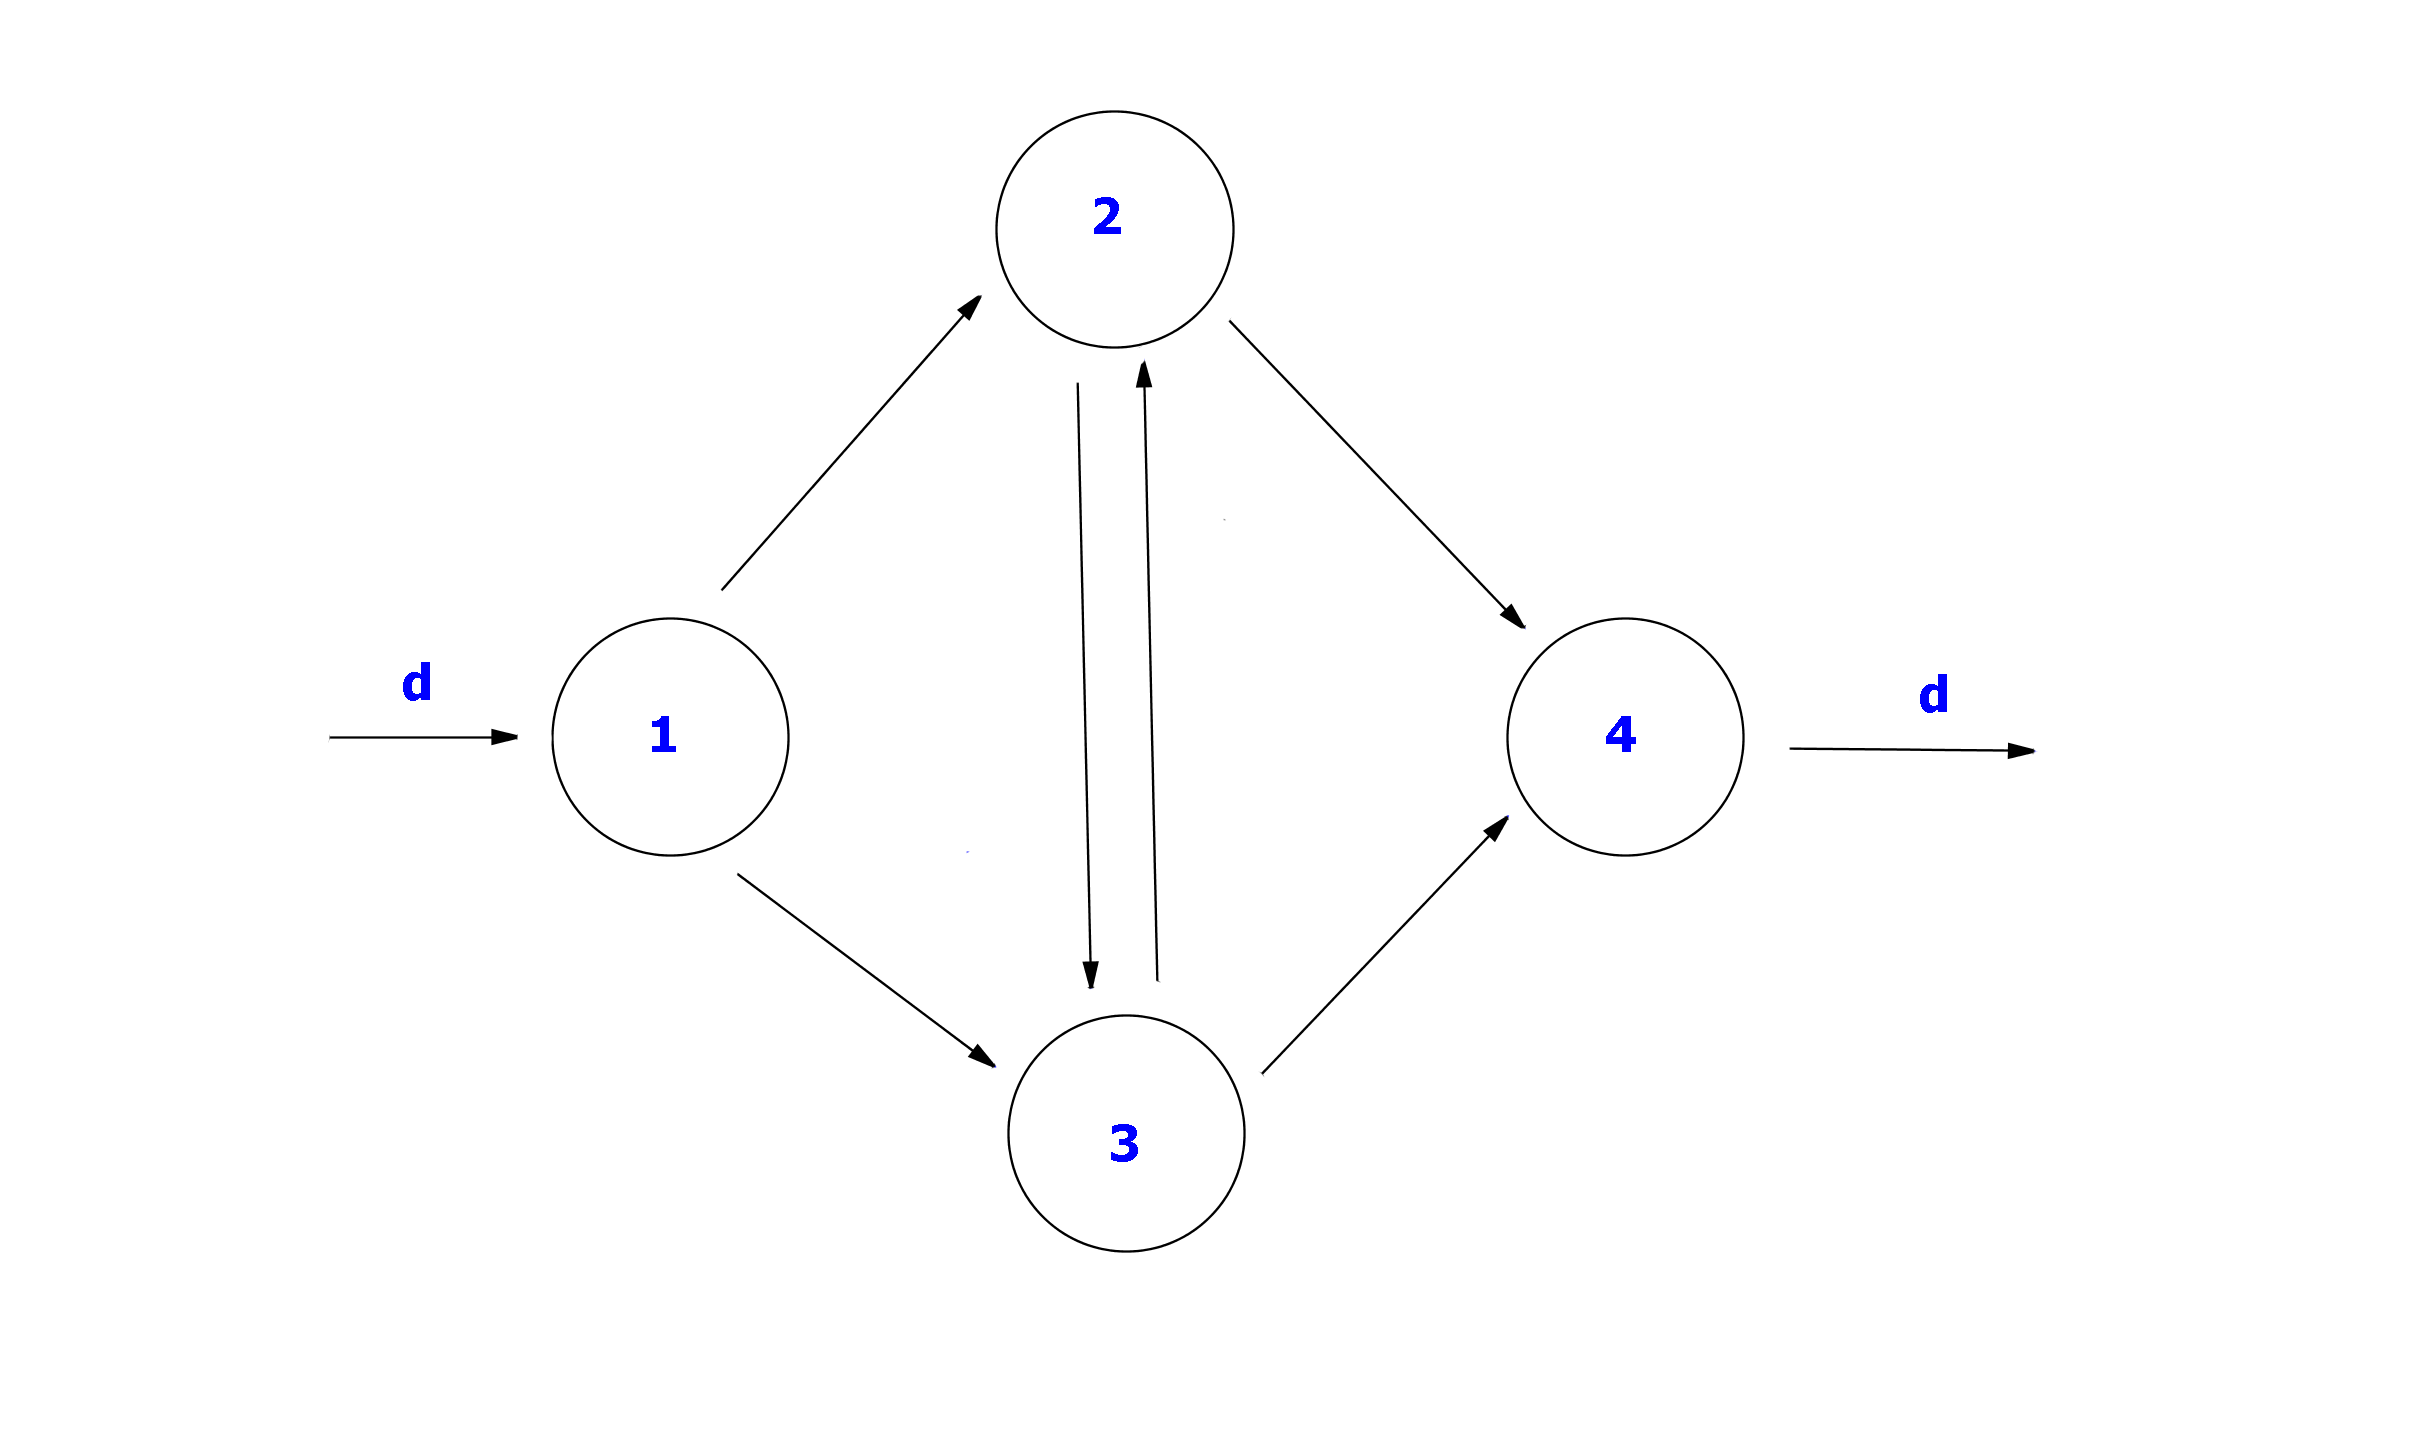
\includegraphics[scale=0.6]{imgs/traffico.png}
\end{center}

Un esempio di funzione che descrive la quantit\`a di tempo necessaria a percorrere
l'arco $ij$ \`e la seguente:
$$
t_{ij}(v) = t_{ij} + \alpha _{ij}  \frac{v}{c_{ij} - v} \quad  (v < c_{ij}) \qquad
\left \{
\begin{array}{ll}
 t_{ij}, \alpha _{ij} & \text{ costanti relative al tipo di strada} \\
 c_{ij}: & \text{ capacit\`a  in } ij \\
 v:  & \text{ volume di traffico attuale} 
\end{array}
\right.
$$
Un'altra funzione possibile per descrivere il tempo di attraversamento al variare del volume 
di traffico \`e 
$$
t_{ij}(v) = t_{ij} + \alpha_{ij} \dfrac{v_j}{c_{ij}^{4}}
$$
dove $c_{ij}$ non \`e la capacit\`a!
La funzione obiettivo da minimizzare \`e:
$$ \min \displaystyle \sum_{(i,j)} x_{ij} t_{ij} (x_{ij}) $$
Il problema questa volta \`e  vincolato:  abbiamo dei vincoli di conservazione del flusso
ossia, la quantit\`a di traffico che entra da un nodo deve essere uguale a quella che esce.\
La regione ammissibile \`e descritta da:
$$
\left\{
\begin{array}{l}
x_{12} + x_{13} = d               \\
x_{24} + x_{34} =d                \\
x_{12} + x_{32} = x_{23} + x_{24} \\
x_{13} + x_{23} = x_{32} + x_{34} \\
x_{ij} \geq 0                     \\
 (x_{ij} \leq c_{ij}) \quad  (\text{opzionale: capacit\`a limitata su un arco})
\end{array}
\right.
$$
Il problema pu\`o essere descritto pi\`u in generale dalla seguente notazione
basata su grafi:
$$
\displaystyle
\sum_{j \in BN(i)} x_{ji}
-
\displaystyle
\sum_{j \in FN(i)} x_{ji}
=
\left\{
\begin{array}{cl}
  -d & i = 0                      \\
  0  & i \neq 0,t                 \\
  d  & i = t
\end{array}
\right.
$$
\end{example}

\section{Condizioni di ottimalit\`a con regione ammissibile convessa}
Come facciamo a sapere se l'insieme \`e convesso?
$$ X = \{ x \in \mathbb{R}^{n} \; : \; g_{i}(x) \leq 0, h_j(x)=0 \} $$
$$
i=1\ldots n \quad j=1\ldots p
\quad
g_i : \mathbb{R}^{n} \rightarrow \mathbb{R}
\quad
h_i : \mathbb{R}^{n} \rightarrow \mathbb{R}
$$
Le funzioni $g_i$ (vincoli di disuguaglianza) e $h_j$ (vincoli di
uguaglianza) definiscono i vincoli applicabili su $\mathbb{R}^n$ per
definire la regione ammissibile.
La natura delle funzioni vincolari pu\`o garantire la convessita di $X$.
% Quando riusciremo ad avere un insieme convesso?

\begin{defn}[Funzione affine]
Una funzione $h_j$ si dice \emph{affine} se
$$ h_j(x) = a_{j}^{T}x + b_j
\qquad
a_j \in \mathbb{R}^{n}, b_j \in \mathbb{R}
$$
\end{defn}

\begin{proposition}
Se le funzioni $g_i$ sono convesse per $i=1\ldots n$ e le funzioni
$h_j$ sono affini per $j=1\ldots p$, allora $X$ \`e un insieme convesso
\end{proposition}
\begin{thproof}
Si sfrutta la definizione di convessit\`a. Si prendano
$x,y \in X$ e $\lambda \in [0,1]$.
Il segmento che unisce i due punti \`e dato da
$$ \lambda x + (1- \lambda )y$$
\begin{itemize}
\item Vincoli di disuguaglianza:
$$ g_i(\lambda x + (1-\lambda) y)
\leq
\lambda \underbracket{ g_i(x)}_{\leq 0}
+ (1- \lambda) \underbracket{ g_i(y)}_{\leq 0}
\; \leq \;  0
$$
\begin{notes}
$g_i(x) \leq 0$ e $g_i(y) \leq 0$ in quanto per ipotesi apparengono ad
$X$: se non fosse cos\`i $x$ ed $y$ sarebbero fuori dalla regione
ammissibile.
\end{notes}
\item
Vincoli di uguaglianza:
$$
\begin{array}{lr}
  h_j(\lambda x + (1-\lambda)y) = & \\
  a_j^{T}(\lambda x + (1-\lambda)y)+ b_j = & [\; \text{ponendo } b_j = 
  \lambda b_j + (1-\lambda) b_j  \; ]   \\
  \lambda a_{j}^{T}x + (1-\lambda) a_{j}^{T}y+ 
  \lambda b_j + (1-\lambda) b_j = \\
  \lambda \underbracket{h_j(x)}_{=0} + (1-\lambda) \underbracket{h_j(y)}_{=0} = 0
\end{array}
$$
\begin{notes}
$g_i(x) = 0$ e $g_i(y) =  0$ in quanto per ipotesi apparengono ad
$X$.
\end{notes}
\end{itemize}


\end{thproof}
Per avere un algoritmo, dobbiamo stabilire le condizioni di ottimalit\`a:
minimo locale e globale. \\
L'ipotesi che assumiamo \`e che $f$ sia differenziabile, in modo
che si possano utilizzare i gradienti e le matrici hessiane. \\
Le condizioni di ottimalit\`a che abbiamo visto nel caso non vincolato,
valgono anche nel caso vincolato?

\begin{example}
Vediamo in esempio in cui dimostriamo che le condizioni di ottimalit\`a
viste nel caso non vincolato non sono pi\`u sufficienti.
Vogliamo minimizzare la funzione
$$ f(x) =  x_1^{2} + x_2^{2}
\qquad
X = [1,2] \times [0,1]
$$
\begin{center}
  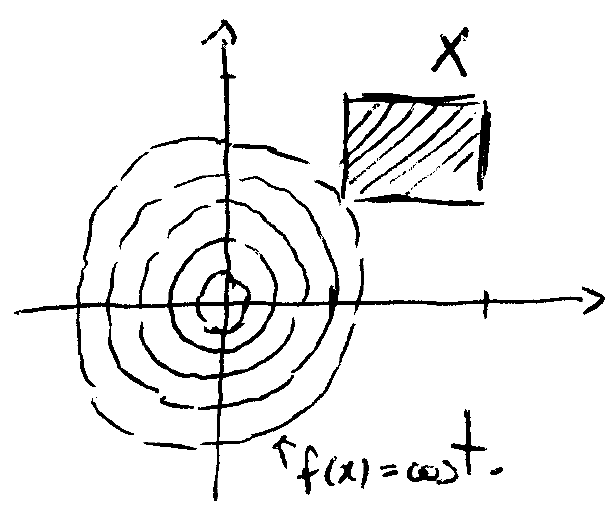
\includegraphics[width=0.3\textwidth]{imgs/vincolocos.png}
\end{center}

Nel caso non vincolato il minimo \`e in $(0,0)$
ed il gradiente di $f$ \`e
$$ \nabla f(x) = 2x$$
Il gradiente si annulla nel caso del vettore $x=0$,
ma $x \notin X$.
\end{example}

Questo esempio quindi dimostra che
questa non pu\`o essere la condizione di ottimalit\`a:
bisogna cercare una differente nozione di punto stazionario.

\begin{defn}[Direzione ammissibile]
Un vettore $d \in \mathbb{R}^{n}$ si dice
\emph{direzione ammissibile} per
$X$ a partire da $\overline{x} \in X$
se  $\exists \overline{t} > 0 \text{  tale che  }$
$$
x(t) = \overline{x} + td \in X \quad
\forall t \in [0,\overline{t}]
$$
\end{defn}
Se $d$ \`e una direzione ammissibile, anche i suoi
multipli sono ancora una direzione ammissibile.\\
L'insieme in cui appartengono anche i suoi multipli
si chiama \emph{cono}.

\begin{defn}[Cono delle direzioni ammissibili]
$$ F(X, \overline{x}) = \{
d \in \mathbb{R}^{n}\; : \;
\exists \overline{t}> 0 \; \text{tale che} \;
\overline{x} + td \in X \quad \forall t \in [0,\overline{t}] \; \}
$$
\end{defn}

\begin{observation}
Se $d$ appartiene alla regione ammissibile, anche tutti i suoi multipli ci appartengono.
\end{observation}

\begin{observation}
Se $\overline{x}$ \`e un punto \emph{interno} a $X$, allora
$$F(X,\overline{x}) = \mathbb{R}^{n}$$
\end{observation}

L'idea quindi \`e quella di testare l'ottimalita lungo tutte
le direzioni ammissibili.

\begin{theo}[Condizione necessaria]
\label{ottvinc:01}
 Sia $\overline{x} \in X$  un punto di minimo locale per $(P)$.
Allora
$$ \nabla f(\overline{x})^{T} d \geq 0 \quad
\forall d \in F(X,\overline{x}) \qquad (CN_{F}) $$
Che \`e detta condizione di stazionariet\`a. ($F(X,\overline{x}$ sono le direzioni ammissibili)
\end{theo}
% Un punto pu\`o essere punto di minimo locale solo se il gradiente
% si annulla.

\begin{thproof}
Sia $\epsilon > 0 $ tale che 
$f(\overline{x}) = \min \{ f(x) \; : \; x \in X \cap B(\overline{x}, \epsilon) \;\}$ e sia $ d \in F(X, \overline{x})$ con $\overline{t} > 0$
fornito dalla definizione. Considerando
$t \leq \min\{ \dfrac{\epsilon}{||d||_2}, \overline{t} \}$, risulta
$\overline{x} + td \in X \cap B(\overline{x}, \epsilon)$ e quindi
$f(\overline{x}, + td) - f(\overline{x}) \geq 0$.
A questo punto si procede come nel caso non vincolato,
utilizzando lo sviluppo di Taylor
$$ 0 \leq
\dfrac{ f(\overline{x} + td) - f(\overline{x})}{t} = 
\nabla f(\overline{x})^{T}d + \dfrac{r(td)}{t} 
\xrightarrow{t \downarrow 0} \nabla f(\overline{x})^{T}d
$$
e quindi $\nabla f(\overline{x})^{T}d \geq 0$
% $$ 0 \underbracket{\leq}_{\text{punto critico}} f(\overline{x} + td) - f(\overline{x}) =
% t \nabla f(\overline{x})^{T} d + r(td)
% $$

% $$ 0 \leq f(\overline{x})^{T} d +
% \dfrac{r(td)}{t} \quad \xrightarrow{t\rightarrow 0^{+}}
% \quad
% \nabla f(\overline{x})^{T} d
% $$
\end{thproof}

Il teorema contiene al suo interno come caso particolare
l'ottimizzazione non vincolata, infatti:
$$ X = \mathbb{R}^{n} \quad \Rightarrow \quad
F(X,\overline{x}) = \mathbb{R}^{n}$$
$$ \overline{x} \text{ punto min. loc.} \quad \Leftrightarrow \quad \nabla f(\overline{x}) =0\quad \Rightarrow \quad \nabla f(\overline{x})^T d \geq 0
$$
Se un punto \`e stazionario per $f$ ed appartiene
alla regione ammissibile, soddisfa la condizione necessaria
di ottimalit\`a.

\begin{observation}
  \begin{enumerate}
  \item Se $\nabla f(\overline{x})=0$, allora $(CN_{F})$ \`e verificata
  \item Se $x \in intX$ \`e un punto di minimo locale di $(P)$, allora
    $\nabla f(\overline{x}) = 0$
  \end{enumerate}
\end{observation}

\begin{proposition}
  \label{prop:cono-convesso}
  Sia $X$ un insieme \emph{convesso}, $\overline{x} \in X$. Allora
  \begin{enumerate}
  \item $x -\overline{x}$ \`e una direzione ammissibile per $X$ per
    ogni $x \in X$.
  \item Se $d \in F(X, \overline{x})$, allora esistono $\lambda \geq 0,
    x \in X$ tali che $d = \lambda(x - \overline{x}) $
  \end{enumerate}
  Da 1 e 2 segue che il cono delle direzioni ammissibili è
  $$ F(X, \overline{x}) = \{ \lambda(x -\overline{x}) \; : \;
  \lambda \geq 0, x \in X \} $$ 
\end{proposition}

\begin{thproof}
  \begin{enumerate}
  \item Sia $ \in [0,1]: \overline{x} + t(x -\overline{x}) = 
  (1-t) \overline{x} + tx \in X $ poich\`e $X$ \`e convesso.
  Allora $(x - \overline{x}) \in F(X, \overline{x})$ 
 \item Sia $t > 0$ tale che $\overline{x} + td \in X$.
 Posto  $x = \overline{x} + td \in X$, risulta 
$ d = \dfrac{1}{t}(x - \overline{x})$
  \end{enumerate}
\end{thproof}
Segue da questa caratterizzazione del teorema 1 una riscrittura

\begin{theo}[Condizione necessaria (2)]
  Sia $X$ convesso, $\overline{x} \in X$.
  Se $\overline{x} \in X$ \`e un punto di minimo locale
  per $(P)$, allora
  $$ \nabla f(\overline{x})^{T}(x - \overline{x}) \geq 0
  \quad \forall x \in X \qquad (CN_{X})$$
  Viceversa, se $f$ \`e convessa, $\overline{x} \in X$, e vale la
  condizione di stazionariet\`a $(CN_{X})$, allora $\overline{x}$ \`e un
  punto di minimo (globale) di (P).
\end{theo}
$(CN_{X})$ è una condizione necessaria, se $f$ è convessa diventa
anche sufficiente, questo perch\`e minimo locale e globale coincidono.

\begin{thproof}
La prima parte viene da (\ref{ottvinc:01}) 
(\ref{prop:cono-convesso}.2), la seconda parte va dimostrata.

$x \in X$. La funzione $f$ \`e convessa: se $f$ \`e differenziabile
e convessa vale (caratterizzazione delle funzioni convesse)
$$ f(x) \underbracket{\geq}_{f \text{convessa}}
f(\overline{x}) + {\nabla f(\overline{x})^{T}(x- \overline{x})}
\underbracket{\geq}_{CN_x} f(\overline{x})
$$
\end{thproof}
\begin{figure}[h!]
 \centering
 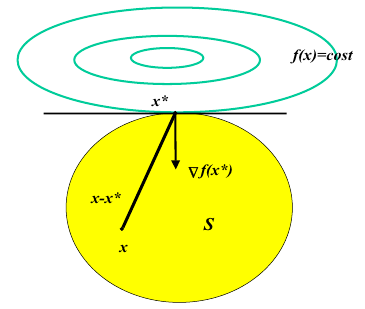
\includegraphics[width=0.4\textwidth]{./imgs/ottvinc08.png}
 % ottvinc08.png: 365x309 pixel, 96dpi, 9.66x8.18 cm, bb=0 0 274 232
 \caption{Significato geometrico della condizione necessaria di ottimalit\`a}
\end{figure}

\begin{workinprogress}
  Digressione: compagnie telefoniche (minimi quadrati).  Gauss Newton
$$
J_{k}^{T}J_{k} + \displaystyle \sum_{j=1}^{n} r_{j} (x^{k})
\nabla^{2}r_j(x^{k})
$$
\end{workinprogress}

%% 5 Aprile
\section{Metodi risolutivi}

%\subsection{Metodi per regioni ammissibili convesse generiche}
Ora che abbiamo il concetto di stazionarietà con vincolo, possiamo
ridefinire il punto stazionario.

\begin{defn}[Punto stazionario]
  Un punto $\overline{x} \in X$ si dice \emph{stazionario} se
  $$ \nabla f(\overline{x})^{T}d \geq 0 \quad \forall  d \in F(X, \overline{x})$$
  % $$(\text{se X convesso}
  % \Rightarrow F(X,\overline{x}) =
  % \{ \lambda (x -\overline{x}) : x \in X, \lambda \geq 0 \}$$
\end{defn}
L'ipotesi che useremo sempre \`e che $X$ sia \emph{convesso}, con la
semplificazione \ref{prop:cono-convesso}.\\

Dobbiamo muoverci per punti ammissibili, quindi direzioni ammissibli e
di discesa.
Quindi:
\begin{itemize}
\item Direzione di discesa \quad $\nabla f(x^k)^Td^k < 0$
\item Direzione ammissibile \quad $d^k \in F(X,x^k)$
\end{itemize}

\subsection{Metodi delle direzioni ammissibili}
Una assunzione che facciamo, oltre alla convessit\`a della regione
ammissible, \`e che da una direzione, muovendosi di passo unitario, si
rimanga nella regione ammissibile.
$$ x^k + t_k d^k \in X $$
Questa assunzione non \`e restrittiva in quanto se con passo unitario
si uscisse dalla regione ammissibile, si pu\`o sempre scalare
accorciando la direzione stessa moltiplicandola per un coefficiente
minore di 1.\\
Questo consente di restringere la ricerca del passo $t_k \in \left (
0,1\right ]$.\\
Una possibile ricerca del passo di ricerca pu\`o essere quella di
prendere un passo che soddisfi la condizione di Armijo, la quale ci
permette di forzare il valore della funzione obiettivo di una certa
quantit\`a nel nuovo punto.

\begin{defn}[Condizione di Armijo (AJO)]
  $$ f(x^k +td^k) \leq f(x^k) + c_1 t \nabla f(x^k)^Td^k \qquad
  c_1 \in (0,1) $$
\end{defn}
\begin{observation}
  $t_k \in (0,1]$ va bene perch\'e
  $$ X \text{ convesso}  \quad \Rightarrow \quad x^{k} + t_kd^{k} = 
  (1-t_k)x^{k} + t_k(x^{k} + d^{k}) \in X$$
\end{observation}
Poich\`e $\nabla f(x^k)^Td^k$ \`e negativo, stiamo forzando il valore
della funzione obiettivo nel nuovo punto a diminuire di una quantit\`a
pari a $c_1 t \nabla f(x^k)^Td^k$.\\

Sappiamo anche che $\exists \tau \ge 0$ tale che vale (AJO)
$\forall t \in (0,\tau]$
$$( \gamma_k(t) = f(x^{k} + td^{k}) \quad \Rightarrow \quad
\gamma_k'(0)  = \nabla f(x^{k})^{T} d^{k}<0 )  $$

\begin{thproof}
  Consideriamo la funzione di ricerca monodimensionale funzione della sola $t$
  \[\begin{array}{ll}
    \varphi (t) &= f(x^k + td^k) \\
    \varphi'(t) &= \nabla f(x^k+td^k)d^k \\
    \varphi'(0) &= \nabla f(x^k)d^k < 0
  \end{array}\]
  $$ 0 > \nabla f(x^k)d^k = \varphi '(0) = 
  \lim_{t \to \infty}\frac{f(x^k + td^k) - f(x^k)}{t} $$
  Visto che la derivata in zero è negativa allora vale la condizione (AJO).
\end{thproof}


\paragraph{Procedura di Armijo}

\begin{center}
\fbox
{
  \begin{minipage}[position]{0.85\textwidth}
    \begin{enumerate}
    \item Secegliere $\gamma \in (0,1); t = 1$
    \item Se $t$ soddisfa (AJO), STOP, $(t_k=t)$
    \item $t= \gamma t$ e ritornare a 2.
    \end{enumerate}
  \end{minipage}
}
\end{center}
Alla fine risulta che $t= \gamma ^S$ con S numero di iterazioni
effettuate. Quindi $\gamma ^{S-1}$ non soddisfa la condizione
(AJO). \\
Quello che ci servir\`a sar\`a (nella dimostrazione della
convergenza?)  appunto che $\displaystyle \frac{t_k}{\gamma}$ non
sar\`a uno spostamento corretto.

Riassumiamo la procedura totale
\paragraph{Procedura per Metodi delle direzioni ammissibili}
\begin{center}
  \fbox{
    \begin{minipage}[position]{0.85\textwidth}
      \begin{enumerate}
      \item Scegliere $x^{0} \in X ; k=0$
      \item Se $\nabla f(x^{k})^{T}d \geq 0 \quad
        \forall d \in F(X,x^{k})$, allora STOP
      \item Scegliere $d^{k} \in F(X, x^{k})$ tale che
        $\nabla f(x^{k})^{T} d^{k} < 0$ e $x^{k} + d^{k} \in X$
      \item Calcolare $t_k \in (0,1]$ che soddisfa (AJO) tramite Procedura di Armijo
      \item $x^{k+1} = x^{k} + t_k d^{K}$
      \item $k=k+1$ e ritornare a 2)
      \end{enumerate}
    \end{minipage}
  }
\end{center}

\begin{observation}
Come caso particolare in cui $X = \mathbb R^n$ ritorniamo ai metodi
del gradiente visti per l'ottimizzazione non vincolata.
\end{observation}

Questa procedura descrive un insieme di metodi che poi si
differenziano in
\begin{itemize}
\item come verificare la condizione di stazionarietà (ora andrebbe
  testata su infinite di direzioni)
\item come scegliere una direzione ammissibile che sia anche di discesa.
\end{itemize}

\begin{property}
  \label{prop:gradiente-compatto}
  Supponiamo che $X$ sia \emph{compatto}. Allora
  $$ \lim_{k \to +\infty} \nabla f(x^{k})^{T}d^{k} = 0 $$
\end{property}
Notare che la condizione di compattezza esclude il caso non vincolato.


\begin{thproof}
  Se vale la condizione di Armijo su $t_k$ allora
  \[\begin{array}{ll}
    f(x^{k}) - f(x^{k}+td^k) &\geq - c_1 t_k \nabla f(x^{k})^{T} d^{k} \\
    f(x^{k}) - f(x^{k+1})    &\geq - c_1 t_k \underbracket{\nabla f(x^{k})^{T} d^{k}}_{negativo}\\
    f(x^{k}) - f(x^{k+1})    &\geq  c_1 t_k | \nabla f(x^{k})^{T} d^{k}|
  \end{array}\]

  X \`e compatto, quindi $f$ su $X$ ammette minimo, quindi
  $\{f(x^{k})\}$ è una successione decrescente, limitata inferiormente,
  che converge. Passando al limite $f(x^k)$ e $f(x^{k+1})$ convergono
  allo stesso valore, da cui:
  $$ \lim_{k \to +\infty}f(x^{k}) - f(x^{k+1}) = 0 $$

  Da cui deduciamo che:
  $$ \lim_{k \to +\infty} t_k | \nabla f(x^{k})^{T}d^{k}| = 0 $$

  quindi una delle due componenti deve essere nulla.\\
  Supponiamo per assurdo che la seconda componente sia diversa da zero:
  $$ \lim_{k \to +\infty}\text{inf } |\nabla f(x^{k})^{T}d^{k}| \geq \eta > 0
  \quad \Rightarrow \quad t_k \to 0 $$
  Abbiamo preso il minimo limite, dato che il limite potrebbe non esistere.\\
  Adesso sfruttiamo la compattezza di $X$: una successione dentro un compatto ammette
  una sottosuccessione convergente .\\
  Inoltre
  $$ \{x^{k}\} \subseteq X, \qquad x^{k} + d^{k} \in X \quad
  \Rightarrow \quad 
  \{ d^{k}\} \text{ \`e limitata }$$

  Quindi entrambe hanno una sottosuccessione convergente:
  $$ x^{k} \rightarrow \overline{x} \qquad d^{k} \rightarrow \overline{d}$$
  (Abbiamo omesso gli indici delle sottosuccessioni). \\
  Il prodotto scalare
  $$\nabla f(x^{k})^{T}d^{k} \rightarrow \nabla f(\overline{x})^{T}\overline{d}
  \leq - \eta < 0$$
  (In quest'ultimo passaggio abbiamo usato la continuit\`a del gradiente
  e del prodotto scalare).\\
  Importante risultato \`e che il prodotto scalare fra il gradiente e la
  direzioni calcolato nei punti limite \`e negativo.\\
  Adesso sfruttiamo la ricerca della condizione di armijo. Se $t_k$
  soddisfa (AJO) il passo $ \dfrac{t_k}{\gamma}$ non pu\`o soddisfare.\\
  Deve essere:
  $$ f(x^{k}+ \dfrac{t_k}{\gamma} d^{k}) -
  f(x^{k}) > c_1 \dfrac{t_k}{\gamma} \nabla f(x^{k})^{T}d^{k}$$
  
  Per il teorema del valor medio:
  $$ f(x^{k}+ \dfrac{t_k}{\gamma} d^{k}) - f(x^{k}) = 
  \nabla f(x^{k} + \tau_k d^k)^{T} \dfrac{t_k}{\gamma} d^{k} \qquad 
  \tau_k \in[0,\dfrac{t_k}{\gamma}]$$
  Riprendendo la disuguaglianza che esprime la non soddisfacibilit\`a di (AJO)
  $$ \cancel{\dfrac{t_k}{\gamma}} \nabla f(x^{k} + \tau_k d^k)^{T} d^{k} > 
  \cancel{\dfrac{t_k}{\gamma}} c_1 \nabla f(x^{k})^{T}d^{k} $$
  Quindi
  $$ \nabla f(x^{k} + \tau_k d^{k})^{T} d^{k} > c_1 \nabla f(x^{k})^{T}d^{k}$$
  Passando ai limiti:
  $$ \nabla f(\overline{x})^{T}\overline{d} \geq
  c_1 \nabla f(\overline{x})^{T} \overline{d} $$
  Quindi deve essere
  $$(1 -c_1)\nabla f(\overline{x})^{T} \geq 0$$
  Questo pu\`o accadere solo se $c_1 \geq 1$, ma la condizione
  che utilizzavamo \`e che
  $$ 0 < c_1 < 1 $$
  quindi abbiamo un \emph{assurdo} e deduciamo che 
  $$ | \nabla f(x^k)^{T} d^{k} | = 0 $$
\end{thproof}

\begin{observation}
La ricerca di Armijo pu\`o essere sostituta dalla Minimizzazione
limitata con passo $t \in[0,1]$. \\ $t_k \in argmin \{ f(x^{k} +
td^{k}): t \in [0,1]\}$ trovato grazie alla ricerca esatta.\\ Si pu\`o
riprendere lo stessa dimostrazione del teorema e si usa il $t_k$ di
Armijo.
\end{observation}

I punti oscuri nel metodo delle direzioni ammissibili sono:
\begin{itemize}
  \item Trovare punto ammissibile
  \item Trovare direzione ammissibile
  \item Verificare la condizione di stazionariet\`a
\end{itemize}


\subsection{Algoritmo di Frank-Wolfe (Gradiente condizionato)}
Era stato pensato per le funzioni quadratiche, ma in realt\`a funziona
anche sulle funzioni non quadratiche. \\
\`E un metodo delle direzioni ammissibili cui si impone direzione
$$ d^{k} = \overline{x}^{k} - x^{k} \qquad 
\overline{x}^{k} \in argmin \{\nabla f(x^{k})(x -x^{k}) \; : \; x \in X \}
$$

La verifica della stazionariet\`a \`e immediata:
\begin{itemize}
\item se $\nabla f(x^{k})^{T}(\overline{x}^{k} - x^{k})=0$ (in
  particolare se $\overline{x}^{k}=x^{k}$), allora $x^{k}$ \`e
  un punto stazionario. 
\item in caso contrario
  $\nabla f(x^{k})^{T}d^{k} < 0$ e $x^{k} + d^{k} = \overline{x}^{k} \in X$, 
  cio\`e $d^{k}$ \`e la direzione cercata.
\end{itemize}
\begin{notes}
Si ricordi
$$ \text{X convesso} \quad \Rightarrow \quad 
F(X, x^{k}) = \{ \lambda (x - x^{k}) : x \in X, \lambda \geq 0 \} $$
\end{notes}

Tuttavia, verificare la condizione di stazionarietà \`e un problema di ottimizzazione non vincolata, se pure più semplice di quello di partenza!\\ 
Tuttavia la funzione obiettivo di questo problema risulta \emph{lineare},
infatti poiché 
$$ \nabla f(x^{k})^{T} (x-x^k) = \underbracket{\nabla f(x^{k})^{T}}_{costante} x -
\underbracket{\nabla (x^{k})^{T}x^k}_{costante} $$ 
risulta
$$ argmin \{\nabla f(x^{k})(x -x^{k}) \; : \; x \in X \} \;\equiv\;
   argmin \{\nabla f(x^{k})x \; : \; x \in X \} $$

Inoltre se $X$ \`e un \emph{poliedro} abbiamo un problema di 
\emph{programmazione lineare}.

Notare che in questo modo risolviamo sia il passo 2) che il passo 3) dell'algoritmo.


\begin{theo}[Convergenza]
  Supponiamo che $X$ sia compatto. Allora ogni punto
  di accumulazione di $\{x^{k}\}$ \`e un punto stazionario di (P)
\end{theo}
\begin{thproof}
  Se $x$ è un punto di accumulazione allora $x^k \rightarrow x^{*}$ e
  dato che siamo in un compatto $x^k + d^k \in X$ allora $d^k
  \rightarrow d^{*}$.\\
  Per come abbiamo calcolato $d_k$ deve essere
  $$ \nabla f(x^{k})^{T} d^k \leq \nabla f(x^{k})^{T} (x -x^{k})
  \quad \forall x \in X$$
  Passiamo al limite membro a membro
  $$ \nabla f(x^{*})^{T} d^{*}
  \leq \nabla f(x^{*})^{T}(x-x^{*}) \quad \forall x \in X$$
  Ma per la proposizione \ref{prop:gradiente-compatto} $\nabla
  f(x^{*})^{T} d^{*} = 0$, che è la condizione di stazionariet\`a di $x^{*}$.
\end{thproof}

\begin{notes}
  Dall'esempio visto al calcolatore, si vede che la direzione
  calcolata andr\`a dal punto di partenza fino a un vertice del
  poliedro. Da qui
  prender\'o un punto che sta su questo segmento. \\
  Se il numero dei vertici sono pochi, si ha una convergenza lenta
  dovuta all'andamento "zig-zag" fra i vertici.
\end{notes}


%%% 8 Aprile 2011
\subsection{Metodi del gradiente proiettato}
\paragraph{Proiezione di un insieme convesso}
$$ X \subseteq \mathbb{R}^{n} \text{ convesso }, y \in \mathbb{R}^{n}$$
La proiezione del punto $y$ su $X$ \`e:
\begin{itemize}
\item se $y \in X$ la proiezione \`e $y$ stesso.
\item se $y \notin X$ la proiezione \`e il punto pi\`u vicino a $y$
  che appartiene a $X$.
\end{itemize}

\begin{center}
  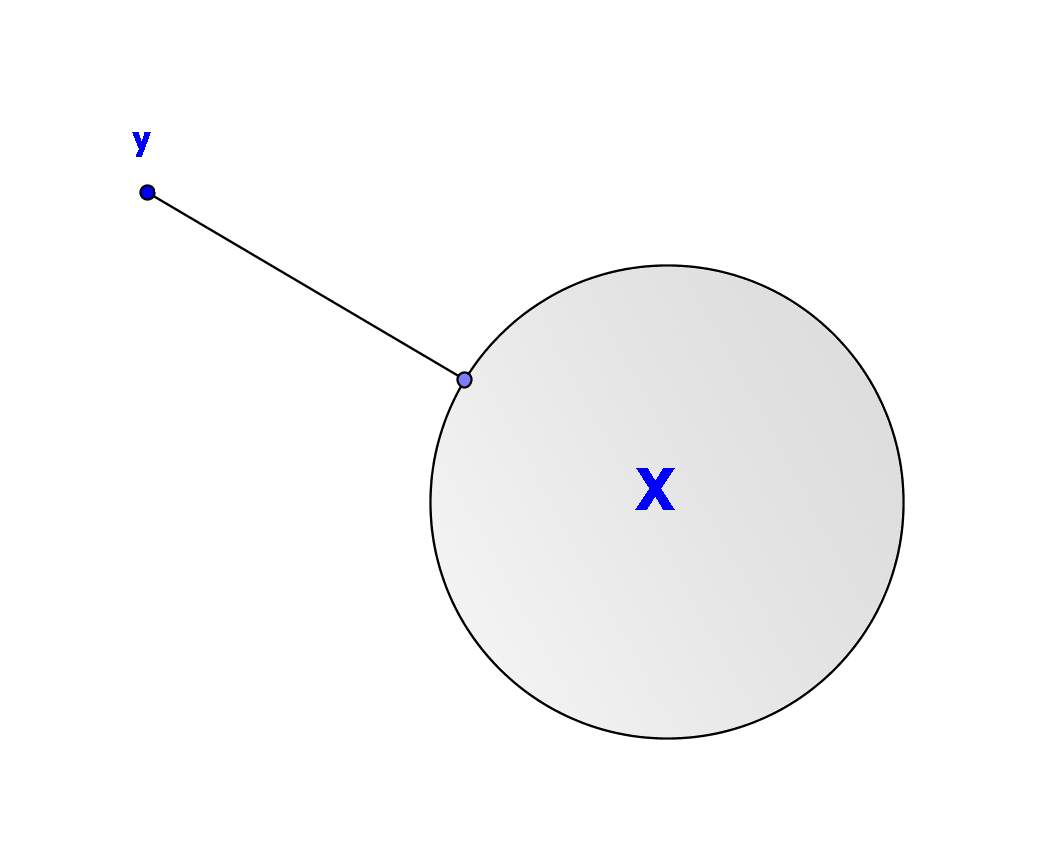
\includegraphics[width=0.4\textwidth]{imgs/proiezione.png}
\end{center}

Per trovare la proiezione dobbiamo risolvere il seguente problema di ottimizzazione:
$$(P_{RX}) \qquad \min \{ || y - x ||_{2} \; : \; x \in X \}$$
Se prendo il quadrato della norma e aggiungo un coefficiente davanti
il problema rimane il medesimo:
$$(P_{RX}) \qquad \min \left\{ \dfrac{1}{2}|| y - x ||_{2}^{2} \}\; : \; x \in X \right\}  $$
Analizziamo la funzione obiettivo, il gradiente e la matrice hessiana
$$ 
\begin{array}{l}
  f(x) = \dfrac{1}{2} || y - x||_{2}^{2} =
  \dfrac{1}{2} \displaystyle \sum_{i=1}^{n} (y_i - x_i)^{2} \\
  \nabla f(x) = x - y \\
  \nabla^{2}f(x) = I \quad (\text{identit\`a})  
\end{array}
$$

La matrice hessiana \`e identica, da questo segue che la
funzione \`e \emph{strettamente} convessa.\\
Dato che $X$ è convesso e $f$ è strettamente convessa esiste un \emph{unico}
minimo: la proiezione \`e unica.

\begin{defn}[Proiezione di $y$ su X]
  $P_{X} : \mathbb{R}^{n} \rightarrow \mathbb{R}^{n}$
  $$P_{X}(y):= argmin \left\{ \dfrac{1}{2} ||x-y||_{2}^{2} : x \in X \right\}$$
\end{defn}

\begin{theo}[Caratterizzazione delle proiezioni]
  \label{ottvinc:050}
  Sia $y \in \mathbb{R}^{n}$ fissato. Allora
  \begin{enumerate}
  \item $x^{*} = P_{X}(y) \quad
    \Longleftrightarrow \quad
    (y - x^{*})^{T} (x - x^{*}) \leq 0 \quad \forall x \in X$
  \item
    $ ||  P_{X}(v) - P_{X}(z)||_{2} \leq ||v-z||_{2} \quad \forall v, z \in \mathbb{R}^{n}$\\
  \end{enumerate}
\end{theo}

\begin{observation}
La caratterizzazione 1) sta ad indicare che
 Il vettore $x - p(x)$ deve formare un angolo maggiore o eguale a $\pi/2$ con ogni vettore
$y - p(x)$, al variare di $y$ in $S$.
\end{observation}
\begin{figure}[h!]
 \centering
 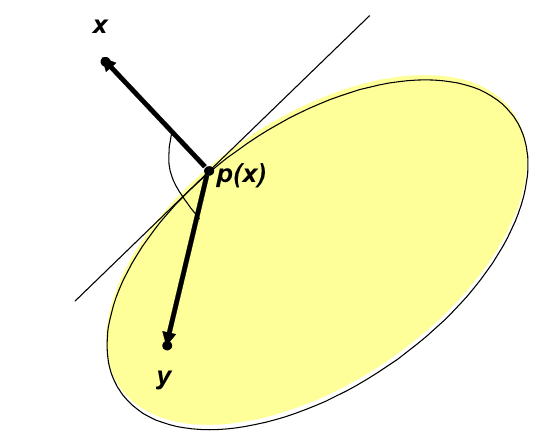
\includegraphics[width=0.4\textwidth]{./imgs/ottvinc09.png}
 % ottvinc09.png: 545x445 pixel, 96dpi, 14.42x11.77 cm, bb=0 0 409 334
 \caption{Significato geometrico della caratterizzazione 1)}
\end{figure}

\begin{observation}
  Da 2) segue che $\lim_{v \to z} P_{X}(v) = P_{X}(z)$, ossia $P_{X}$
  \`e continua.\\ 
  Una funzione così fatta viene anche chiamata non espansiva, cioè una
  funzione così fatta al massimo ``accorcia'' le distanze fra i punti.
\end{observation}

\begin{thproof}
  \begin{enumerate}
  \item $$ x^{*} = P_{X}(y) \quad \Longleftrightarrow \quad
    x^{*} \text{ \`e punto di minimo di } (P_{RX}) $$
    Quindi dalla definizione di minimo:
    $$ \nabla f(x^{*})^{T} (x - x^{*}) \geq 0 \quad \forall x \in X $$
    Andando a sostituire il valore del gradiente precedentemente calcolato
    \[\begin{array}{l}
      (x^{*} - y)^{T} (x - x^{*}) \geq 0 \; \forall x \in X \\
      (y - x^{*})^{T} (x - x^{*}) \leq 0 \; \forall x \in X
    \end{array}\]

  \item indichiamo con $v^{*} = P_{X}(v)$ e $z^{*} = P_{X}(x)$.\\
    Sfruttando la propriet\`a 1)
    
    \[\begin{array}{l}
      (v - v^{*})^{T} (x - v^{*}) \leq 0 \\
      (z - z^{*})^{T} (x - z^{*}) \leq 0 
    \end{array}\]
    Le disuguaglianza sopra valgono $\forall x \in X$ quindi in
    particolare valgono per $x=z^*$ e $x=v^*$.
    \[\begin{array}{l}
      (v - v^{*})^{T} (z^{*} - v^{*}) \leq 0 \\
      (z - z^{*})^{T} (v^{*} - z^{*}) \leq 0 
    \end{array}\]
    Portiamo fuori il meno nella seconda
    \[\begin{array}{l}
      (v - v^{*})^{T} (z^{*} - v^{*}) \leq 0 \\
      - (z - z^{*})^{T} (z^{*} - v^{*}) \leq 0 
    \end{array}\]

    Sommiamo membro a membro (distributiva del prodotto scalare)
    $$
    \begin{array}{c}
      (v - v^{*} - z + z^{*})^{T}(z^{*} - v^{*}) \leq 0 \\
      (v - z)^{T}(z^* - v^*) + \underbrace{(z^* - v^*)^{T}(z^* -
        v*)}_{||z^* - v^*||_2} \leq 0 \\
      || z^{*} - v^{*}||_{2}^{2} + (v - z)^{T}(z^{*} - v^{*}) \leq 0 \\
      || v^{*} - z^{*}||_{2}^{\cancel{2}} \leq
      (v - z)^{T} (v^{*} - z^{*}) \underbracket{\leq}_{*)}
      ||v - z ||_{2} \cancel{||v^{*} -z^{*}||_{2}}
    \end{array}
    $$
    *) per la disuguaglianza di Schwartz
  \end{enumerate}
\end{thproof}

Abbiamo introdotto le proiezioni e analizzato le loro proprietà allo
scopo di utilizzare per l'ottimizzazione vincolata, un metodo non
vincolato, e nel caso si esca dalla regione ammissibile, sia possibile
rientrare dentro con una proiezione.\\
Come abbiamo visto calcolare una proiezione è a sua volta un problema
di ottimizzazione vincolata tuttavia esistono proiezioni che si
riescono a calcolare facilmente, come nei seguenti casi.

\begin{example}[Vincoli di scatola]
$X \in \{ x \in \mathbb{R}^{n} : l_i \leq x_i \leq \mu_i \}
\quad
i =1 \ldots n
$\\
Ogni componente $x_i$ \`e pu\'o variare fra un limite inferiore e un limite superiore.\\
3 casi:
lati esterni, lati superiori, vertici..

\begin{center}
  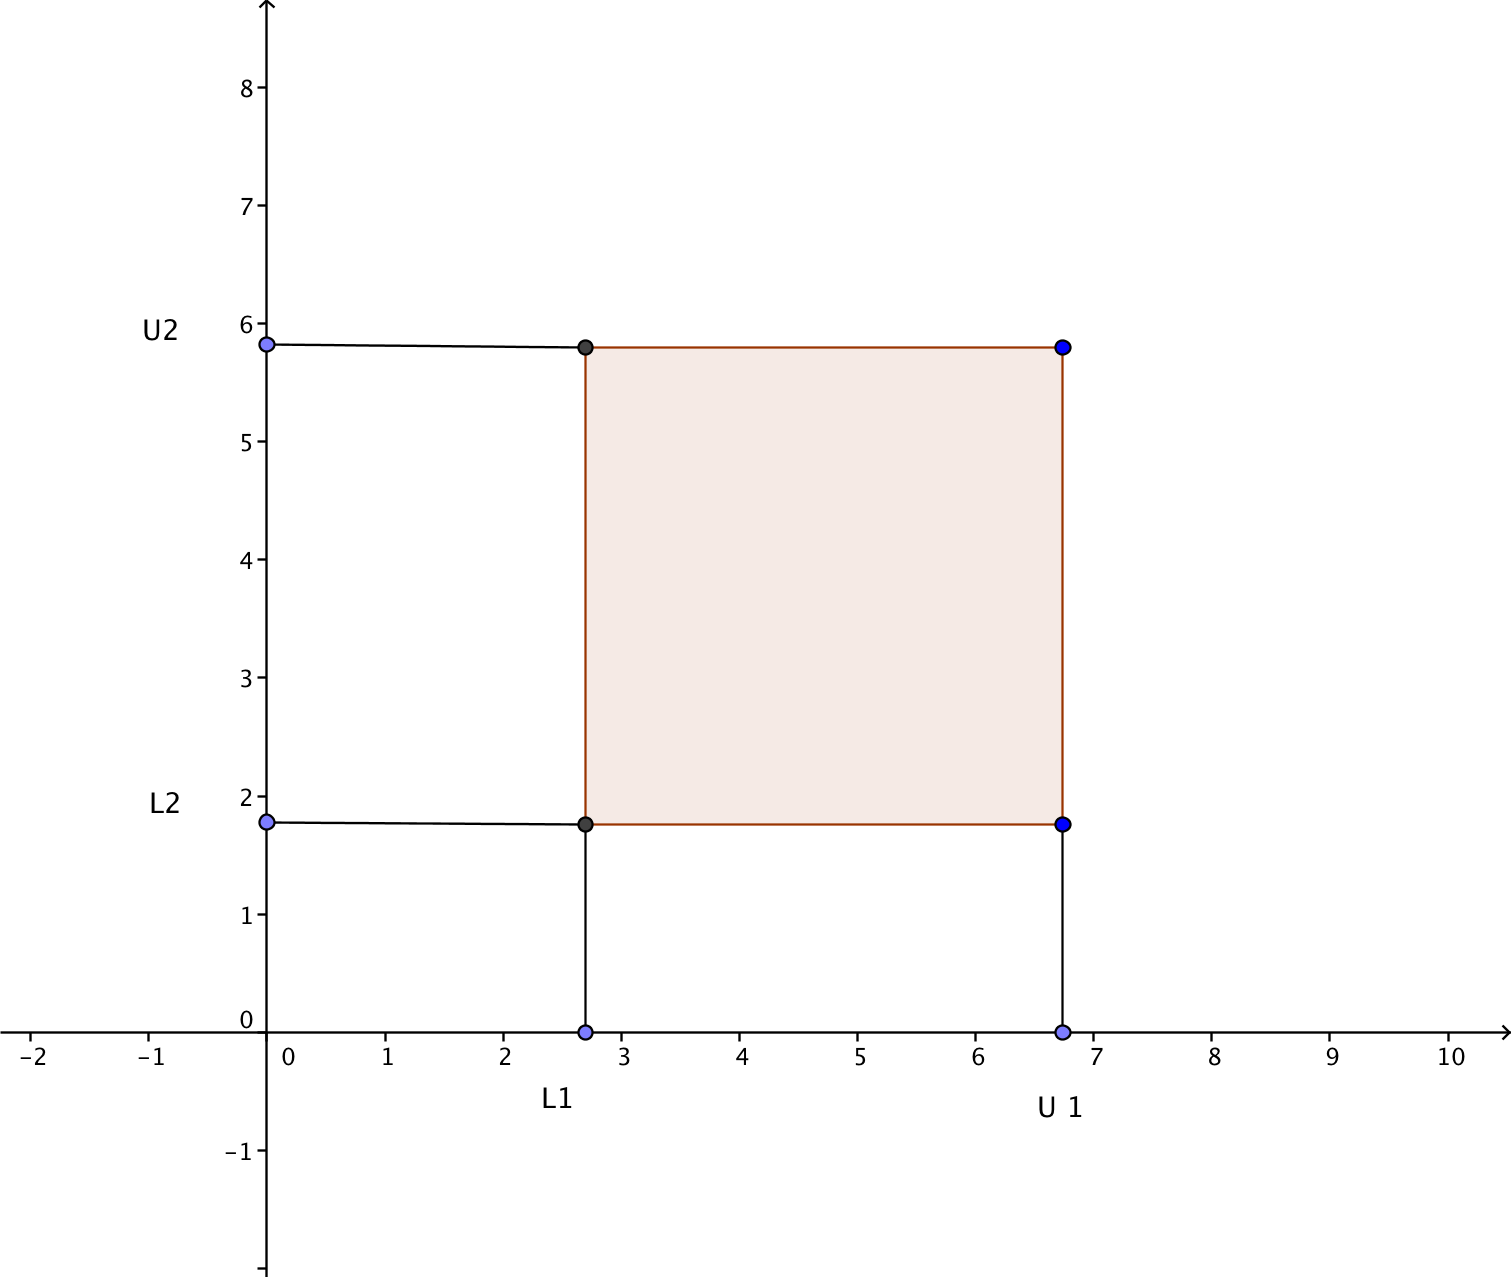
\includegraphics[scale=0.8]{imgs/vincoloscatola.png}
\end{center}


$$[P_{X} (y)]_{i} =
\left\{
\begin{array}{ll}
\mu_i & \text{se } y_i \geq \mu_i \\
l_i & \text{se } y_i \leq l_i \\
y_i & \text{se } l_i \leq y_i \leq u_i \\
\end{array}
\right.
$$
$$
\begin{array}{l}
(y - P_{X}(y))^{T}(x- P_X(y) = \\
\displaystyle \sum_{i=1}^{n}(y_i - [P_x(y)]_{i})(x_i-[P_{X}(y)]_i)
= \\
 \displaystyle \sum_{i \in I_{>}}
\underbracket{(y_i - \mu_i)}_{\geq 0} \underbracket{(x_i - \mu_i)}_{\ge 0}
+
\displaystyle \sum_{i \in I_{<}}
\underbracket{(y_i - l_i)}_{\le 0} \underbracket{(x_i - l_i)}_{\geq 0}   
\; \forall x \in X \quad (I_{>} = \{ i \; | \; y_i > \mu_i \}, \;
I_{<} = \{ i \; | \; y_i < l_i \} )
\end{array}
$$
\end{example}

\begin{example}[Unico vincolo lineare]
$$X_1 = \{ x \in \mathbb{R}^{n} : a^{T}x= b \}$$

\begin{center}
  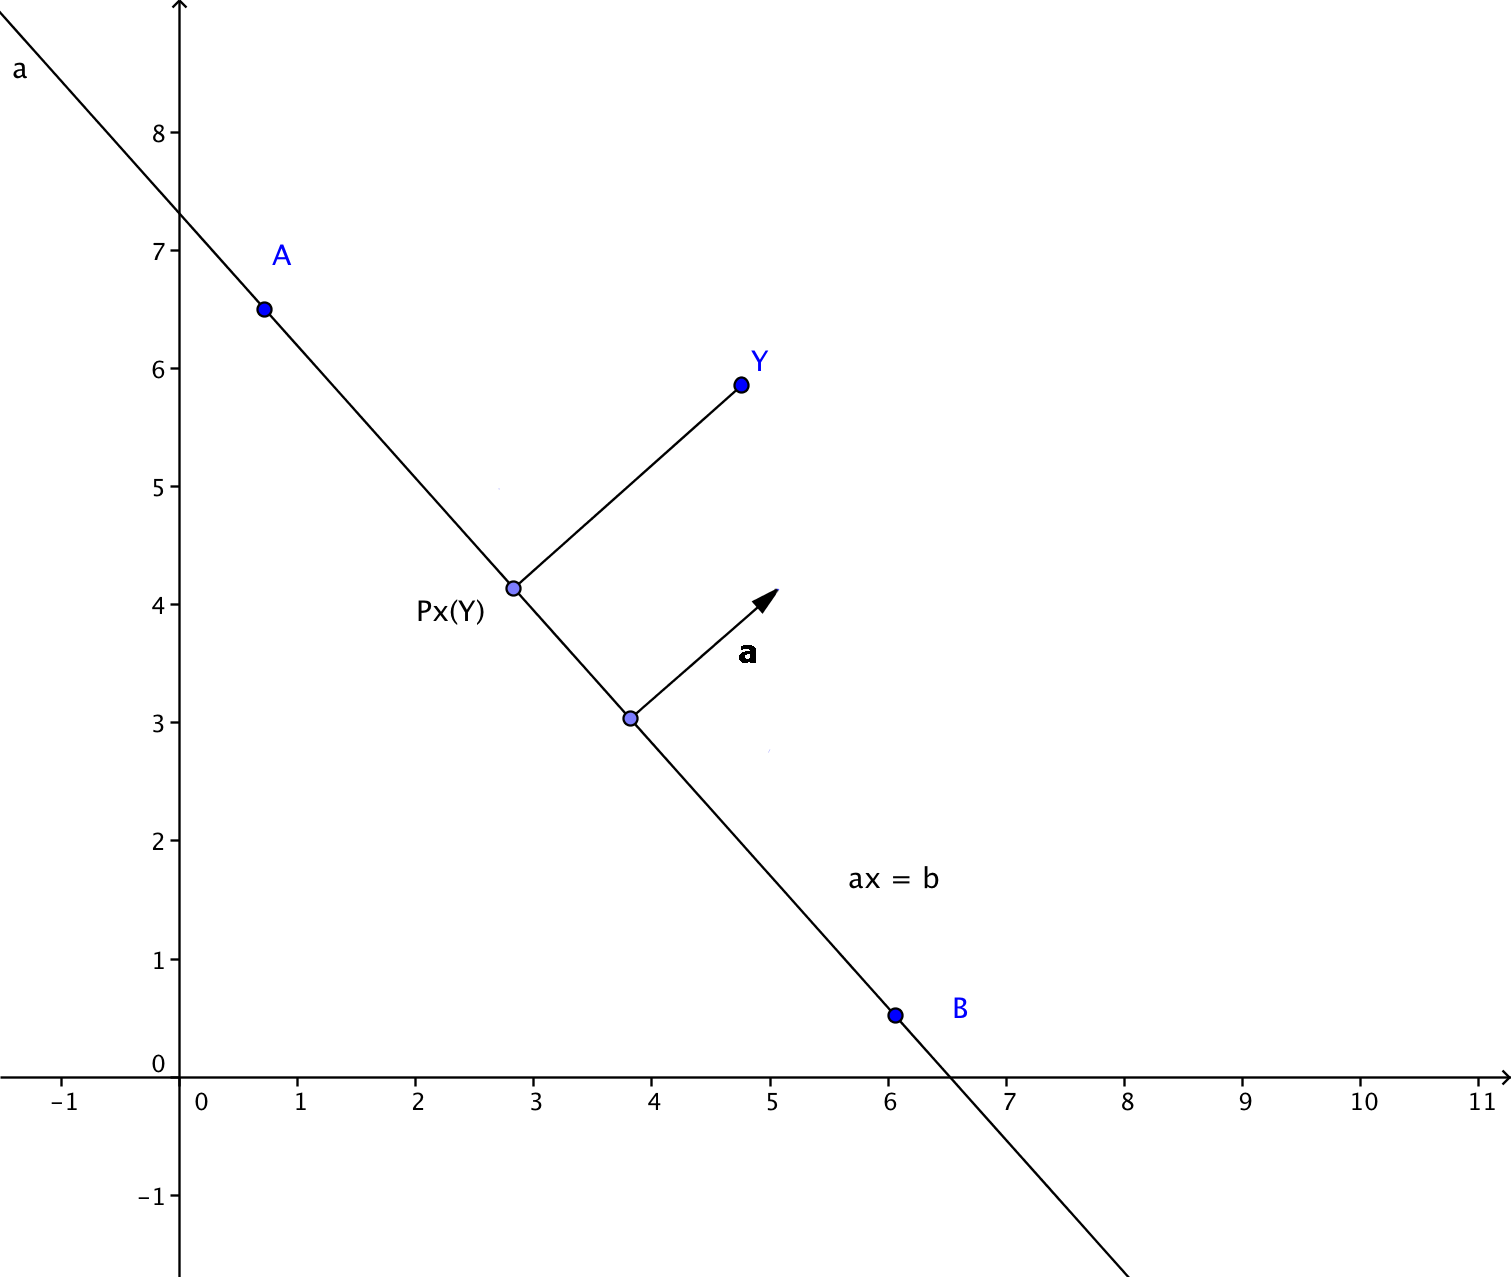
\includegraphics[width=0.45\textwidth]{imgs/vincololineare.png}
\end{center}

Vettore $a$ ortogonale alla retta. Mi sposto da $x$ in una direzione $\pm a$.
\\
$$
P_{X_i}(y) = y - \lambda_i a \qquad
\lambda_1 = \dfrac{a^{T}y-b}{a^{T}a} \quad 
\lambda_2 = \max\{0, \lambda_1\} = \dfrac{1}{a^{T}a}\max\{0,a^{T}x-b\}$$

$$
\begin{array}{l}
 y - [y - \lambda_ia])^{T}(x - [y -\lambda_i a]) =  \\
\lambda_i a^{T}(x - y + \lambda_i a) =  \\
\lambda_i (a^{T}x - a^{T}y) + \lambda_i^{2} a^{T}a = 
\left\{
\begin{array}{ll}
 = \dfrac{(b -a^{T}y)(a^{T}y-b)}{a^Ta} + \dfrac{(a^{T}y -b)^{2}}{a^{T}a}=0
\quad & \forall x \in X_1 \\
\leq \lambda_1[(b-a^{T}y -b ) + (a^{T}y -b)] = 0 \quad & \forall 
x \in X_2
\end{array}
\right.  
\end{array}
$$
Nel secondo caso lo spostamento \`e
$$X_2 = \{ x \in \mathbb{R}^{n} : a^{T}x \leq  b \}$$

\begin{center}
  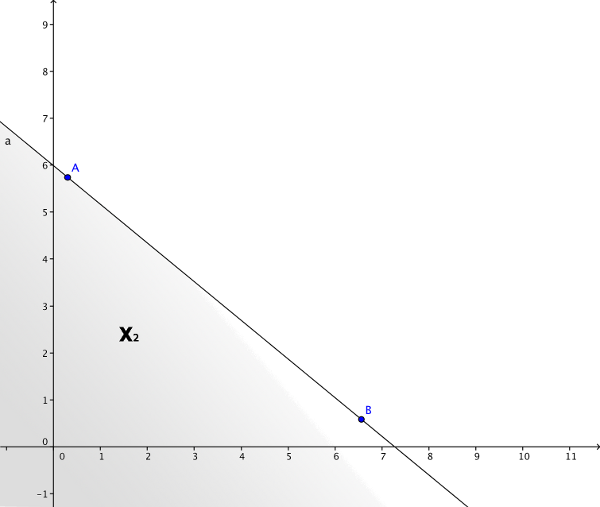
\includegraphics[width=0.3\textwidth]{imgs/vincololineare2.png}
\end{center}
Se sono dentro la regione ammissibile, lo spostamento \`e 0. Altrimenti se sono fuori scelgo $\lambda _1$ che sar\`a $ > 0$ dato che $a^{T}y > 0$
Tutto questo discorso vale solo con un vincolo lineare.
\end{example}

\begin{example}[Sfera]
$$
X  = \{ x \in \mathbb{R}^{n} \; : \;
|| x - \overline{x}||_{2} \leq r \} = B(\overline{x},r)
$$

\begin{center}
  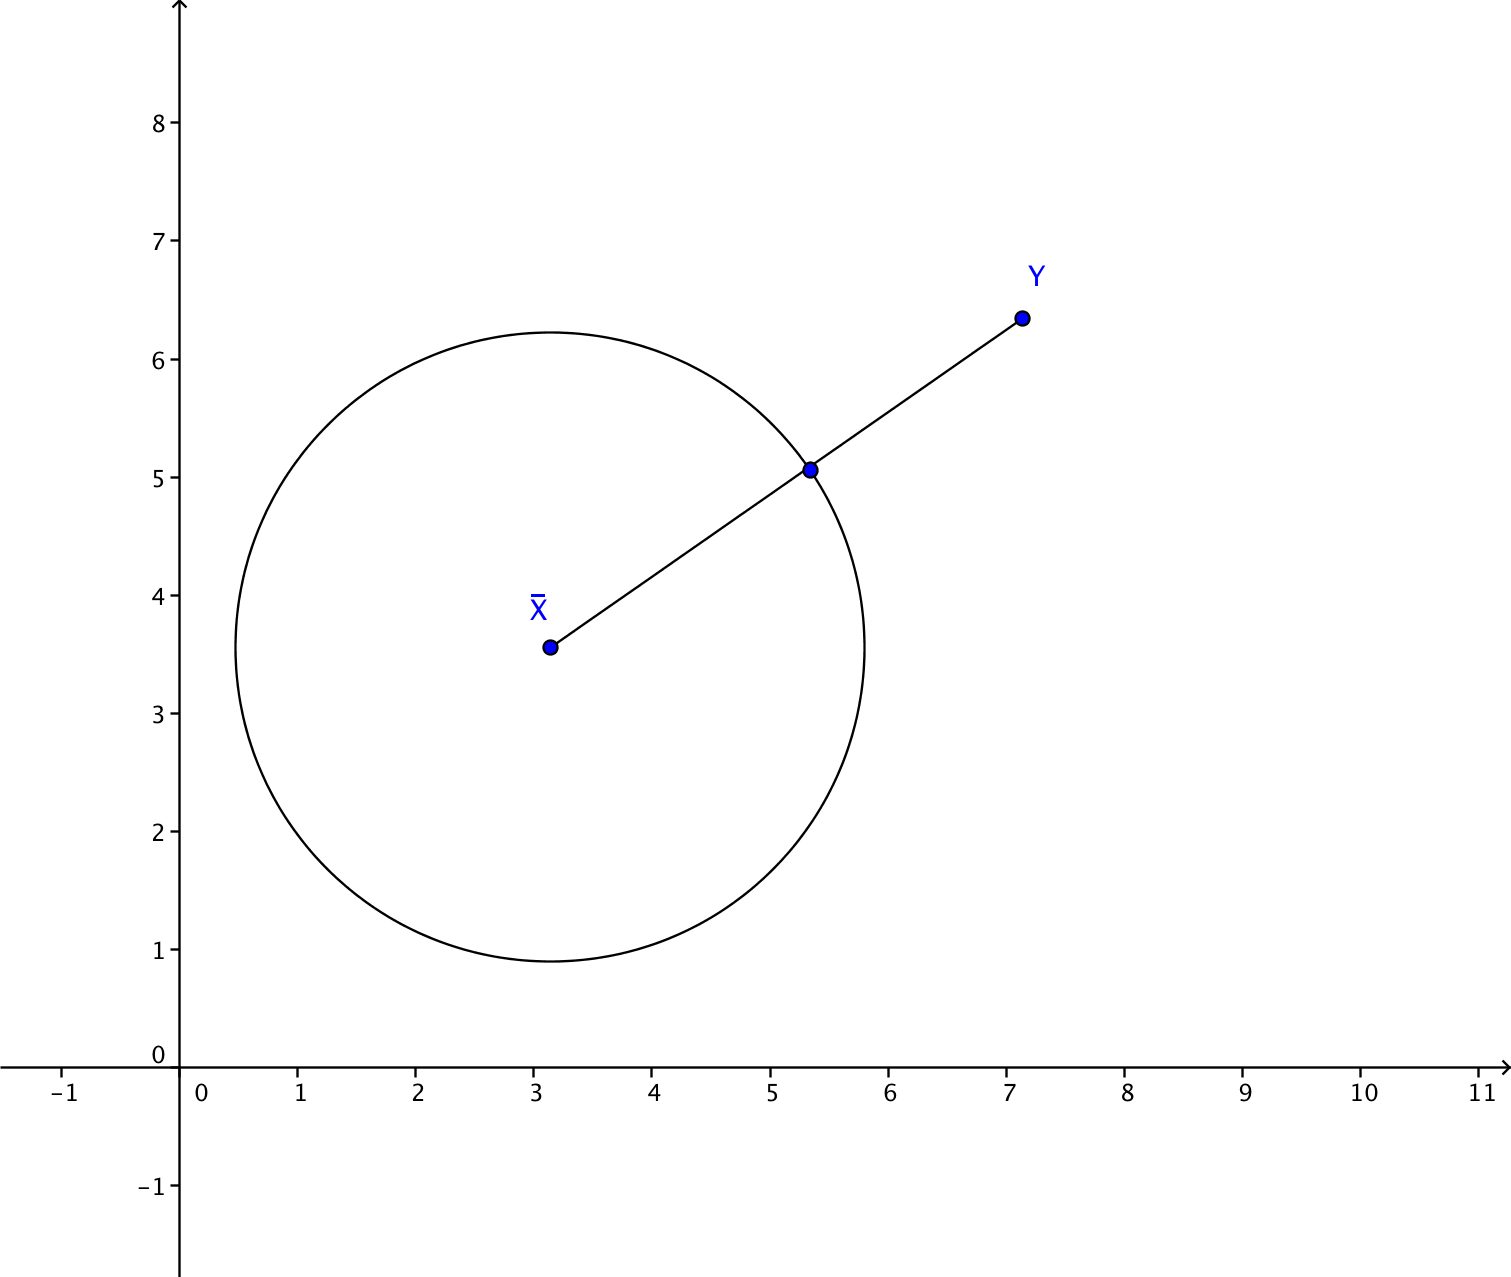
\includegraphics[scale=0.6]{imgs/sferavincolo.png}
\end{center}

La proiezione \`e verso il centro.
Se sono dentro non ci si deve spostare.

$$P_{X}(y) = \overline{x} + \underbracket{(\min \{ || y - \overline{x}||_{2},r\})}_{\lambda} =
\dfrac{y-\overline{x}}{||y - \overline{x} ||_{2}}
$$
Tramite una translazione dall'origine possiamo supporre $\overline{x}=0$
$$
\begin{array}{l}
|| y||_{2} (y - \dfrac{\lambda y}{ ||y||_{2}})^{T}
(x - \dfrac{\lambda y}{ ||y||_{2}}) = 
(||y||_{2} - \lambda) (y^{T}x - \lambda ||y||_{2})
\underbracket{\leq}_{\text{Schwarz}} \\
\leq (||y||_{2}-\lambda)(||y||_{2} ||x||_{2} - \lambda||y||_{2})
= ||y||_{2} (||x||_{2} - \lambda \underbracket{\leq}_{(*)} 0 
\end{array}
$$
$ (*) \lambda <r \; \Rightarrow \lambda = ||y||_{2} \; ; \;
\lambda = r \; \Rightarrow \; ||y|_{2} \geq \lambda \text{ e }
||x||_{2} \leq \lambda 
 $
\end{example}

\subsection{Metodo del gradiente proiettato}
Il metodo consiste nell'applicare il metodo del gradiente e, nel caso
si esca dalla regione ammissibile, di proiettarlo su $X$.

$$ (P) \quad  \min \{ f(x) \; : \; x \in X \}
\qquad
X \subseteq \mathbb{R}^{n} \text{convesso, }
f:\mathbb{R}^{n} \rightarrow \mathbb{R}^{n}
\text{ differenziabile con continuit\`a}
$$

\`E un metodo delle direzioni ammissibili in cui
$d^{k} = \overline{x}^{k} - x^{k}$
$$ x^{k+1} = x^k + t_k (\overline{x}^k - x^k) $$
$$ \overline{x}^{k} = P_{X}(x^{k} - s_{k} \nabla f(x^{k})) \quad
\text{con } s_k > 0 \text{ il passo}$$
Poich\'e $\overline{x}^{k} \in X$, abbiamo
$x^{k} + d^{k} = \overline{x}^{k} \in X$.
\begin{center}
  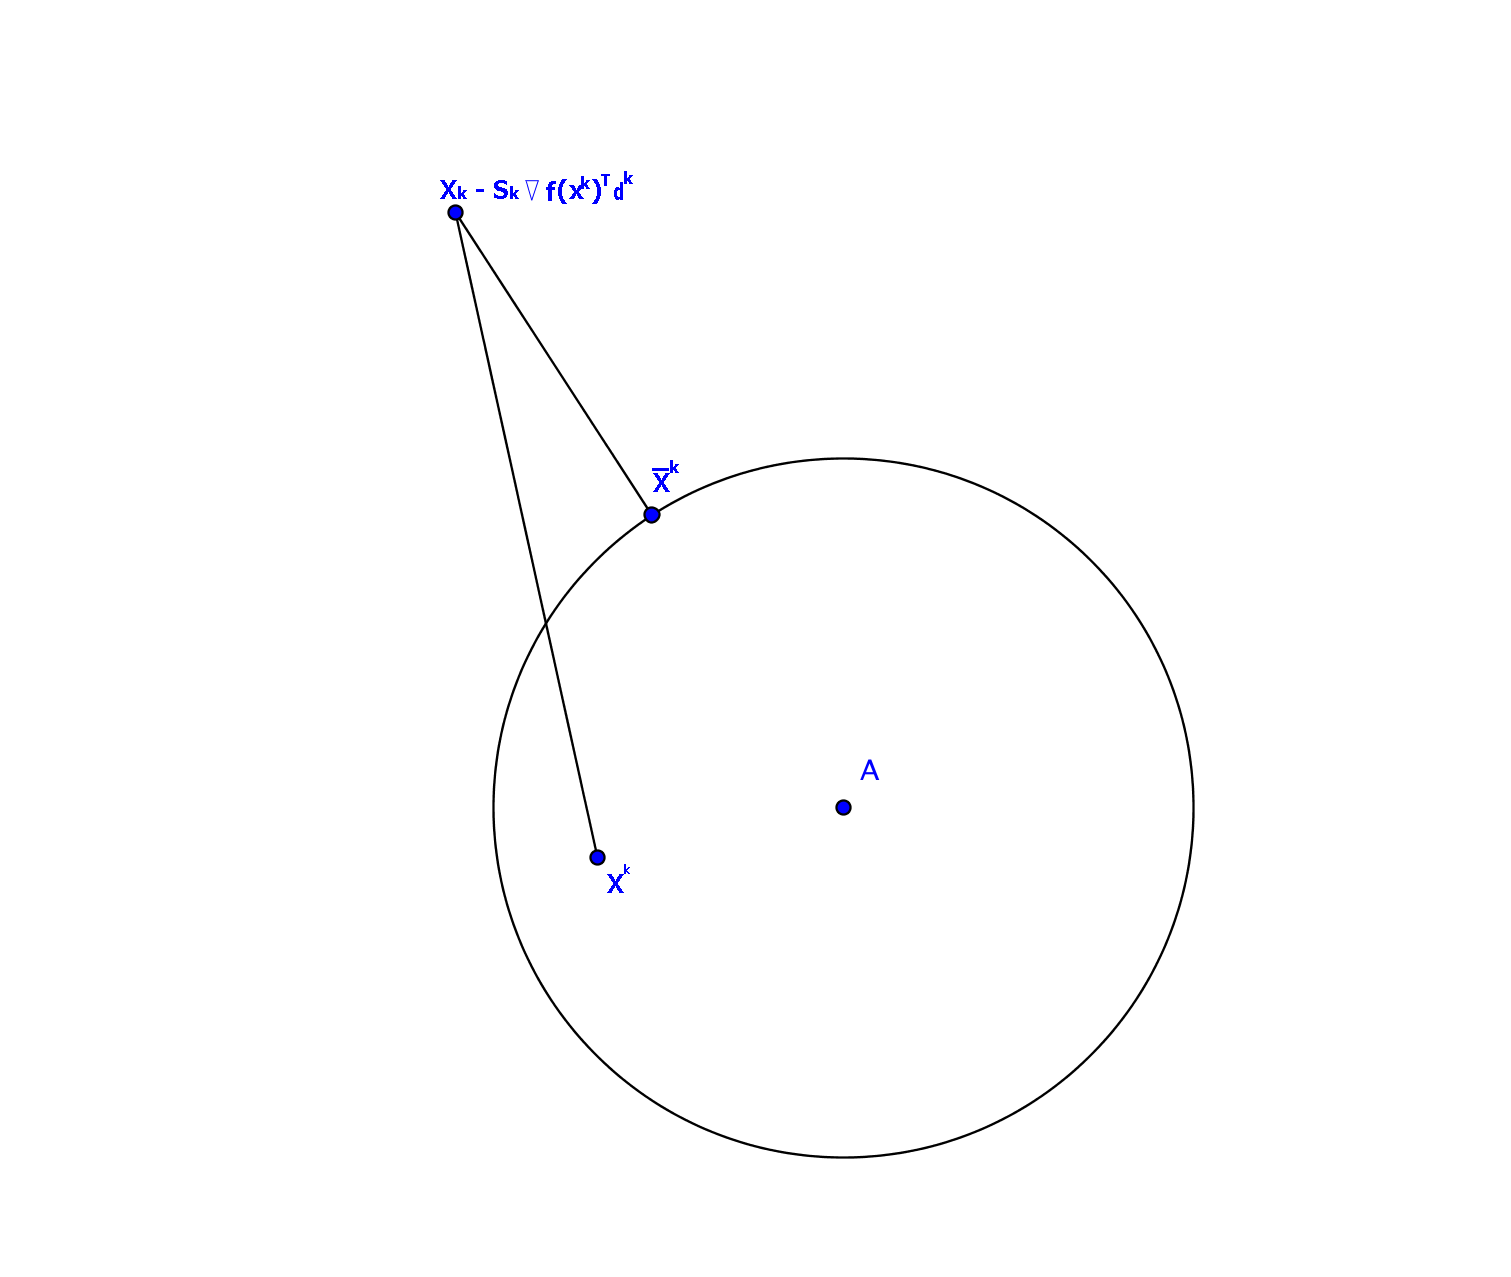
\includegraphics[scale=0.6]{imgs/gradproiettato.png}
\end{center}
Se $x^{k} \neq \overline{x}^{k}$ (cio\`e $d^{k} \neq 0$), allora
$d^{k}$ \`e una direzione di discesa.

\begin{theo}
  $d^{k} = \overline{x}^{k} - x^k$ \`e una direzione di discesa
  (in quanto $\nabla f(x^{k})^{T}d^{k} < 0$).
\end{theo}

\begin{thproof}
Poich\'e $\overline{x}^{k}$ \`e una proiezione, dalla 
caratterizzazione \ref{ottvinc:050}.(1) con $x=x^{k}$ abbiamo
$$
\begin{array}{l}
0 \underbracket{\geq}_{\ref{ottvinc:050}} (x^{k} - s_k \nabla f({x}^{k}) -\overline{x}^{k})^{T}
(x^{k} - \overline{x}^{k}) = s_k \nabla f(x^{k})^{T}
(\overline{x}^{k}- x^{k}) + (x^{k} - \overline{x}^{k})^{T}
(x^{k} - \overline{x}^{k}) = \\
s_k \nabla f(x^{k}) d^{k} + 
|| x^{k} - \overline{x}^{k}||_{2}^{2}   
\end{array}
$$
da cui
$$\nabla f(x^{k})^{T} d^{k} \leq
- \dfrac{1}{s_k} ||x^{k} - \overline{x}^{k}||_{2}^{2} < 0
$$
\end{thproof}
Se invece $\overline{x}^{k} = x^{k}$ (cio\`e $d^{k} = 0$), allora
$x^{k}$ \`e un punto stazionario. Infatti:

\begin{proposition}
\label{prop:proiettato-stazionario}
Sia $s > 0$ fissato. Allora
$$ x^{*} \in X \text{ \`e un punto stazionario di (P) }
\quad \Longleftrightarrow \quad
P_{X}(x^{*} - s \nabla f(x^{*})) = x^{*}
$$
\end{proposition}

\begin{thproof}
$$x^{*} = P_{X} (x^{*} - s\nabla f(x^{*})
\quad
\Longleftrightarrow_{theo di prima}
\quad
(\cancel{x^{*}} - s  \nabla f(x^{*})) \cancel{- x^{*}})^{T}
 (x-x^{*}) \leq 0 \forall x \in X
\quad
\underbracket{\Longleftrightarrow}_{\ref{ottvinc:050}.(1)}
\quad
\cancel{s} \nabla f(x^{*})^{T}\underbrace{(x-x^{*})}_{d^k} \geq 0 \; \forall x \in X
$$
\end{thproof}

\begin{theo}[Convergenza]
Supponiamo che $X$ sia compatto. Se $s_k \in [s, s']$ per ogni $k$
per qualche $s, s'> 0$, allora ogni punto di accumulazione
$x^{*}$ di $\{x^{k}\}$ \`e un punto stazionario di $(P)$.
\end{theo}

\begin{thproof}
Dato che $x^{*}$ è un punto di accumulazione allora esiste una
sottosuccessione di $x^k \rightarrow x^{*}$.\\
Sfruttando la trasformazione usata in una dimostrazione precedente:

$$ || \overline{x}^k - x^k ||_2 = 
|| P_X (x^k - s \nabla f(x^k)) d^k - x^k ||_2 \underbracket{\leq}_{teo \ref{ottvinc:050}}
\cancel{x^k} - s \nabla f(x^k) d^k - \cancel{x^k} 
\xrightarrow{k \to \infty \ref{prop:gradiente-compatto}} 0 $$ 
possiamo fare il limite perché la proiezione è continua, quindi
$$ || P_X (x^{*} - s \nabla f(x^{*})) - x^{*} ||_2 = 0 $$ 
da cui 
$$ x^{*} = || P_X (x^{*} - s \nabla f(x^{*})) $$
e quindi $x^{*}$ è stazionario per \ref{prop:proiettato-stazionario}.\\

Abbiamo posto $s^k=s$ per evitare che andasse all'infito, basta
imporre che sia limitato.

% $$(y-\overline{x}^k)^T(x-\overline{x}^k) \leq 0 \quad \forall x \in X $$
% $$\nabla f(x^{k})^{T} d^{k}
% \leq
%  - \dfrac{1}{s_k}|| x^{k} - \overline{x}^{k}||_{2}^{2} $$
% $$ ||\overline{x}^{k} - x^{k} ||_{2}
% \leq
%  \nabla f(x^{k})^{T}d^{k}
% $$
% Per la lezione scorsa sappiamo
% $$  \nabla f(x^{k})^{T}d^{k} \xrightarrow{k \to +\infty} 0 \quad \Rightarrow \qquad \text{al limite } \quad 0 \leq ||\overline{x}^{k} - x^{k} ||_{2} \leq \rightarrow 0$$
% $$
% || P_{X}(x^{k} - s\nabla f(x^k))-x^{k}||_{2} =
% || \overline{x}^{k} - x^{k} ||_{2}
% $$

% Ma $|| P_{X}(x^{k} - s\nabla f(x^k))-x^{k}||_{2}$
% \`e fatto tutto da funzioni continue (compresa la proiezione).
% quindi
% il limite $x_k \to x^{*}$ \`e la stessa funzione calcolata in $x^{*}$.
% quindi
% $$ || P_{X}(x^{*} -s \nabla f(x^{*}) - x^{*})||_{2}=0$$
% Quindi abbiamo concluso. Notare che \`e stato importante supporre
% che $s_k$ fosse fisso. Se $s_k$ va a infinito, il teorema poteva non valere.\\
% Si potrebbe dimostrare ancora con $s_k$ minore di una costante
% fissata.
\end{thproof}

\begin{center}
\fbox{
	\begin{minipage}[position]{0.85\textwidth}

\begin{enumerate}
\item Scegliere $x^{0} \in X ; s> 0  k=0$
\item Calcolare $x^{k+1} = P_X(x^{k} - s \nabla f(x^{k}))$
\item Se $x^{k+1} = x^{k}$, allora STOP
 \item $k=k+1$ e ritornare a 2
\end{enumerate}
\end{minipage}
}
\end{center}


\paragraph{Cenni sull'originale metodo del gradiente proiettato}
Si pu\`o prendere $t_k$ identicamente 1. (versione originale dell'algoritmo)
$$(x^{k+1} = x^{k} = P_{X}(x^{k} - s_{K}\nabla f(x^{k}))$$
Ma non \`e detto che valga la condizione di Armijo,
non rientra quindi nell'insieme dei metodi delle direzioni
ammissibili e quello che si pu\`o dimostrare
che ottieniamo punti stazionari sotto questa condizione:

\begin{itemize}
\item $X$ compatto
\item $\nabla$ lipschitziana $|| \nabla f(x)  - \nabla f(y)|| \leq L ||x -y ||$
\item $ 0 < s \leq 2/L$
\end{itemize}
Risultato che non dimostriamo: questo metodo richiede la conoscenza
di $L$, e non \`e banale.




\outbpdocument
